
%% Work and Energy Questions used on the
%% NYSED Physics Regents Examination
%%--------------------------------------------------

%% this section contains 109 problems


%% Section June2016
%%--------------------
\element{nysed}{
\begin{question}{June2016-Q12}
    A horizontal force of \SI{20}{\newton} eastward causes a \SI{10}{\kilo\gram} box to have a displacement of \SI{5}{\meter} eastward. 
    The total work done on the box by the \SI{20}{\newton} force is:
    \begin{multicols}{2}
    \begin{choices}
        \wrongchoice{\SI{40}{\joule}}
      \correctchoice{\SI{100}{\joule}}
        \wrongchoice{\SI{200}{\joule}}
        \wrongchoice{\SI{1000}{\joule}}
    \end{choices}
    \end{multicols}
\end{question}
}

\element{nysed}{
\begin{question}{June2016-Q13}
    A block initially at rest on a horizontal,
        frictionless surface is accelerated by a constant horizontal force of \SI{5.0}{\newton}.
    If \SI{15}{\joule} of work is done on the block by this force while accelerating it,
        the kinetic energy of the block increases by:
    \begin{multicols}{2}
    \begin{choices}
        \wrongchoice{\SI{3.0}{\joule}}
      \correctchoice{\SI{15}{\joule}}
        \wrongchoice{\SI{20.}{\joule}}
        \wrongchoice{\SI{75}{\joule}}
    \end{choices}
    \end{multicols}
\end{question}
}

\element{nysed}{
\begin{question}{June2016-Q14}
    Two objects, $A$ and $B$, are held one meter above the horizontal ground. 
    The mass of $B$ is twice as great as the mass of $A$. 
    If $PE$ is the gravitational potential energy of $A$ relative to the ground,
        then the gravitational potential energy of $B$ relative to the ground is:
    \begin{multicols}{2}
    \begin{choices}
        \wrongchoice{$PE$}
      \correctchoice{$2PE$}
        \wrongchoice{$\dfrac{PE}{2}$}
        \wrongchoice{$4PE$}
    \end{choices}
    \end{multicols}
\end{question}
}

\element{nysed}{
\begin{question}{June2016-Q15}
    What is the kinetic energy of a \SI{55}{\kilogram} skier traveling at \SI{9.0}{\meter\per\second}?
    \begin{multicols}{2}
    \begin{choices}
        \wrongchoice{\SI{2.5e2}{\joule}}
        \wrongchoice{\SI{5.0e2}{\joule}}
      \correctchoice{\SI{2.2e3}{\joule}}
        \wrongchoice{\SI{4.9e3}{\joule}}
    \end{choices}
    \end{multicols}
\end{question}
}


%% Section June2015
%%--------------------
\element{nysed}{
\begin{question}{June2015-Q42}
    Which combination of fundamental units can be used to express the amount of work done on an object?
    \begin{choices}
        \wrongchoice{kilogram meter per second (\si{\kilo\gram\meter\per\second})}
        \wrongchoice{kilogram meter per second squared (\si{\kilo\gram\meter\per\second\squared})}
      \correctchoice{kilogram meter squared per second squared (\si{\kilo\gram\meter\squared\per\second\squared})}
        \wrongchoice{kilogram meter squared per second cubed (\si{\kilo\gram\meter\squared\per\second\cubed})}
    \end{choices}
\end{question}
}

\element{nysed}{
\begin{question}{June2015-Q48}
    The graph below represents the relationship between the force exerted on an elevator and the distance the elevator is lifted.
    \begin{center}
    \begin{tikzpicture}
        \begin{axis}[
            axis y line=left, 
            axis x line=bottom, 
            axis line style={->},
            xlabel={Distance Lifted},
            x unit=\si{\meter},
            xtick={0,3,6,9},
            xticklabels={$0.0$,$3.0$,$6.0$,$9.0$},
            ylabel={Force Exerted},
            y unit=\SI{e4}{\newton},
            ytick={0,1,2},
            yticklabels={$0.0$,$1.0$,$2.0$},
            xmin=0,xmax=10,
            ymin=0,ymax=2.5,
            width=0.8\columnwidth,
            height=0.5\columnwidth,
            font=\small,
        ]
        \addplot[line width=1pt,domain=0:3]{1.0};
        \addplot[line width=1pt,domain=3:10]{2.0};
        \addplot[dashed] coordinates { (3,1.0) (3,2.0) }; 
        \end{axis}
    \end{tikzpicture}
    \end{center}
    How much total work is done by the force in lifting the elevator from \SI{0.0}{\meter} to \SI{9.0}{\meter}?
    \begin{multicols}{2}
    \begin{choices}
        \wrongchoice{\SI{9.0e4}{\joule}}
        \wrongchoice{\SI{1.2e5}{\joule}}
      \correctchoice{\SI{1.5e5}{\joule}}
        \wrongchoice{\SI{1.8e5}{\joule}}
    \end{choices}
    \end{multicols}
\end{question}
}


%% Section June2014
%%--------------------
\element{nysed}{
\begin{question}{June2014-Q19}
    When a mass is placed on a spring with a spring constant of \SI{60.0}{\newton\per\meter},
        the spring is compressed \SI{0.500}{\meter}.
    How much energy is stored in the spring?
    \begin{multicols}{2}
    \begin{choices}
      \correctchoice{\SI{7.50}{\joule}}
        \wrongchoice{\SI{60.0}{\joule}}
        \wrongchoice{\SI{30.0}{\joule}}
        \wrongchoice{\SI{15.0}{\joule}}
    \end{choices}
    \end{multicols}
\end{question}
}

\element{nysed}{
\begin{question}{June2014-Q48}
    Which graph best represents the greatest amount of work?
    \begin{multicols}{2}
    \begin{choices}
        \AMCboxDimensions{down=-2.5em}
        \correctchoice{
            \begin{tikzpicture}
                \begin{axis}[
                    axis y line=left,
                    axis x line=bottom,
                    axis line style={->},
                    xlabel={distance},
                    xtick={0,0.25,0.5},
                    x unit=\si{\meter},
                    ylabel={force},
                    ytick={0,4,8},
                    y unit=\si{\newton},
                    xmin=0,xmax=0.55,
                    ymin=0.0,ymax=8.2,
                    width=0.85\columnwidth,
                    very thin,
                ]
                \addplot[line width=1pt,domain=0:0.5]{8};
                \end{axis}
            \end{tikzpicture}
        }
        \wrongchoice{
            \begin{tikzpicture}
                \begin{axis}[
                    axis y line=left,
                    axis x line=bottom,
                    axis line style={->},
                    xlabel={distance},
                    xtick={0,0.25,0.5},
                    x unit=\si{\meter},
                    ylabel={force},
                    ytick={0,4,8},
                    y unit=\si{\newton},
                    xmin=0,xmax=0.55,
                    ymin=0.0,ymax=8.2,
                    width=0.85\columnwidth,
                    very thin,
                ]
                \addplot[line width=1pt,domain=0:0.5]{8-(16*x)};
                \end{axis}
            \end{tikzpicture}
        }
        \wrongchoice{
            \begin{tikzpicture}
                \begin{axis}[
                    axis y line=left,
                    axis x line=bottom,
                    axis line style={->},
                    xlabel={distance},
                    xtick={0,0.25,0.5},
                    x unit=\si{\meter},
                    ylabel={force},
                    ytick={0,4,8},
                    y unit=\si{\newton},
                    xmin=0,xmax=0.55,
                    ymin=0.0,ymax=8.2,
                    width=0.85\columnwidth,
                    very thin,
                ]
                \addplot[line width=1pt,domain=0:0.5]{4};
                \end{axis}
            \end{tikzpicture}
        }
        \wrongchoice{
            \begin{tikzpicture}
                \begin{axis}[
                    axis y line=left,
                    axis x line=bottom,
                    axis line style={->},
                    xlabel={distance},
                    xtick={0,0.25,0.5},
                    x unit=\si{\meter},
                    ylabel={force},
                    ytick={0,4,8},
                    y unit=\si{\newton},
                    xmin=0,xmax=0.55,
                    ymin=0.0,ymax=8.2,
                    width=0.85\columnwidth,
                    very thin,
                ]
                \addplot[line width=1pt,domain=0:0.5]{16*x};
                \end{axis}
            \end{tikzpicture}
        }
    \end{choices}
    \end{multicols}
\end{question}
}


%% Section June2013
%%--------------------
\element{nysed}{
\begin{question}{June2013-Q14}
    A spring gains \SI{2.34}{\joule} of elastic potential energy as it is compressed \SI{0.250}{\meter} from its equilibrium position.
    What is the spring constant of this spring?
    \begin{multicols}{2}
    \begin{choices}
        \wrongchoice{\SI{9.36}{\newton\per\meter}}
        \wrongchoice{\SI{18.7}{\newton\per\meter}}
        \wrongchoice{\SI{37.4}{\newton\per\meter}}
      \correctchoice{\SI{74.9}{\newton\per\meter}}
    \end{choices}
    \end{multicols}
\end{question}
}


%% Section June2012
%%--------------------
\element{nysed}{
\begin{question}{June2012-Q13}
    On a small planet, an astronaut uses a vertical force of \SI{175}{\newton} to lift a \SI{87.5}{\kilo\gram} boulder at constant velocity to a height of \SI{0.350}{\meter} above the planet's surface.
    What is the magnitude of the gravitational field strength on the surface of the planet?
    \begin{multicols}{2}
    \begin{choices}
        \wrongchoice{\SI{0.500}{\newton\per\kilo\gram}}
      \correctchoice{\SI{2.00}{\newton\per\kilo\gram}}
        \wrongchoice{\SI{9.81}{\newton\per\kilo\gram}}
        \wrongchoice{\SI{61.3}{\newton\per\kilo\gram}}
    \end{choices}
    \end{multicols}
\end{question}
}

\element{nysed}{
\begin{question}{June2012-Q17}
    How much work is done by the force lifting a \SI{0.1}{\kilo\gram} hamburger vertically upward at constant velocity \SI{0.3}{\meter} from a table?
    \begin{multicols}{2}
    \begin{choices}
        \wrongchoice{\SI{0.03}{\joule}}
        \wrongchoice{\SI{0.1}{\joule}}
      \correctchoice{\SI{0.3}{\joule}}
        \wrongchoice{\SI{0.4}{\joule}}
    \end{choices}
    \end{multicols}
\end{question}
}


%% Section June2011
%%--------------------


%% Section June2010
%%--------------------
\element{nysed}{
\begin{question}{June2010-Q16}
    A \SI{75}{\kilo\gram} bicyclist coasts down a hill at constant speed of \SI{12}{\meter\per\second}.
    What is the kinetic energy of the bicyclist?
    \begin{multicols}{2}
    \begin{choices}
        \wrongchoice{\SI{4.5e2}{\joule}}
        \wrongchoice{\SI{9.0e2}{\joule}}
      \correctchoice{\SI{5.4e3}{\joule}}
        \wrongchoice{\SI{1.1e4}{\joule}}
    \end{choices}
    \end{multicols}
\end{question}
}

\element{nysed}{
\begin{question}{June2010-Q17}
    The diagram below represents a \SI{155}{\newton} box on a ramp.
    Applied force $F$ causes the box to slide from point $A$ to point $B$.
    \begin{center}
    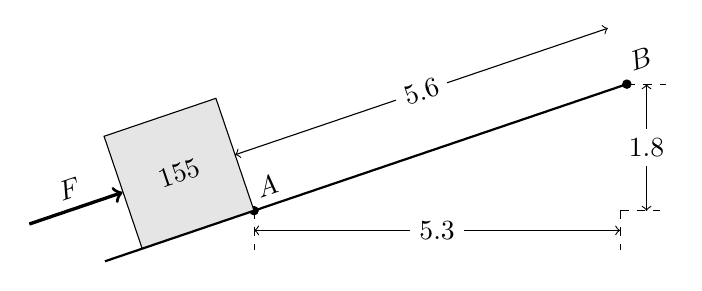
\begin{tikzpicture}
        %% Plane with 18.75865 degree slope
        \draw[thick] (0,0) -- (18.75:7);
        %% Dashes
        \draw[dashed] (18.75:7) -- ++(0:0.5);
        \draw[dashed] (18.75:2) -- ++(270:0.5);
        \draw[dashed] (18.75:2) ++(0:4.65) --++(270:0.5);
        \draw[dashed] (18.75:2) ++(0:4.65) --++(0:0.5);
        %% distance labels
        \draw[<->] (18.75:7) ++(0:0.25) -- ++(270:1.61) node[pos=0.5,anchor=center,fill=white] {\SI{1.8}{\meter}};
        \draw[<->] (18.75:2) ++(270:0.25) -- ++(0:4.65) node[pos=0.5,anchor=center,fill=white] {\SI{5.3}{\meter}};
        \draw[<->] (18.75:2) ++(108.75:0.75) -- ++(18.75:5) node[pos=0.5,anchor=center,fill=white,rotate=18.75] {\SI{5.6}{\meter}};
        %% point A and B
        \draw[fill] (18.75:2) circle (1.5pt) node[anchor=south west,rotate=18.75] {$A$};
        \draw[fill] (18.75:7) circle (1.5pt) node[anchor=south west,rotate=18.75] {$B$};
        %% Box
        \node[draw,fill=white!90!black,anchor=south,rotate=18.75,minimum size=1.5cm] (A) at (18.75:1.25) {\SI{155}{\newton}};
        \draw[very thick,<-] (A.west) -- ++(198.75:1.25) node[pos=0.5,anchor=south,rotate=18.75] {$F$};
    \end{tikzpicture}
    \end{center}
    What is the total amount of gravitational potential energy gained by the box?
    \begin{multicols}{2}
    \begin{choices}
        \wrongchoice{\SI{28.4}{\joule}}
      \correctchoice{\SI{279}{\joule}}
        \wrongchoice{\SI{868}{\joule}}
        \wrongchoice{\SI{2740}{\joule}}
    \end{choices}
    \end{multicols}
\end{question}
}

\element{nysed}{
\begin{question}{June2010-Q36}
    The total work done in lifting a typical high school physics textbook a vertical distance of \SI{0.10}{\meter} is approximately:
    \begin{multicols}{2}
    \begin{choices}
        \wrongchoice{\SI{0.15}{\joule}}
      \correctchoice{\SI{1.5}{\joule}}
        \wrongchoice{\SI{15}{\joule}}
        \wrongchoice{\SI{150}{\joule}}
    \end{choices}
    \end{multicols}
\end{question}
}

\element{nysed}{
\begin{question}{June2010-Q44}
    A \SI{15.0}{\kilo\gram} mass is moving at \SI{7.50}{\meter\per\second} on a horizontal, frictionless surface.
    What is the total work that must be done on the mass to increase its speed to \SI{11.5}{\meter\per\second}?
    \begin{multicols}{2}
    \begin{choices}
        \wrongchoice{\SI{120}{\joule}}
        \wrongchoice{\SI{422}{\joule}}
      \correctchoice{\SI{570}{\joule}}
        \wrongchoice{\SI{992}{\joule}}
    \end{choices}
    \end{multicols}
\end{question}
}


%% Section June2009
%%--------------------
\element{nysed}{
\begin{question}{June2009-Q14}
    The gravitational potential energy, with respect to Earth,
        that is possessed by an object is dependent on the object's:
    \begin{multicols}{2}
    \begin{choices}
        \wrongchoice{acceleration}
        \wrongchoice{momentum}
      \correctchoice{position}
        \wrongchoice{speed}
    \end{choices}
    \end{multicols}
\end{question}
}

\element{nysed}{
\begin{question}{June2009-Q16}
    A spring with a spring constant of \SI{4.0}{\newton\per\meter} is compressed by a force of \SI{1.2}{\newton}.
    What is the total elastic potential energy stored in this compressed spring?
    \begin{multicols}{2}
    \begin{choices}
      \correctchoice{\SI{0.18}{\joule}}
        \wrongchoice{\SI{0.36}{\joule}}
        \wrongchoice{\SI{0.60}{\joule}}
        \wrongchoice{\SI{4.8}{\joule}}
    \end{choices}
    \end{multicols}
\end{question}
}

\element{nysed}{
\begin{question}{June2009-Q36}
    The work done in lifting an apple one meter near Earth's surface is approximately:
    \begin{multicols}{2}
    \begin{choices}
      \correctchoice{\SI{1}{\joule}}
        \wrongchoice{\SI{0.01}{\joule}}
        \wrongchoice{\SI{100}{\joule}}
        \wrongchoice{\SI{1000}{\joule}}
    \end{choices}
    \end{multicols}
\end{question}
}

\newcommand{\myJuneZeroNineQfortyOneTikz}{
\begin{tikzpicture}
    \begin{axis}[
        axis y line=left,
        axis x line=bottom,
        axis line style={->},
        xlabel={distance},
        x unit=\si{\meter},
        xtick={0.0,1.0,2.0,3.0,4.0,5.0,6.0},
        ylabel={force},
        y unit=\si{\newton},
        ytick={0.0,10,20,30,40},
        xmin=0,xmax=6.5,
        ymin=0,ymax=45,
        width=0.8\columnwidth,
        height=0.5\columnwidth,
        very thin,
    ]
    \addplot[line width=1pt,domain=0:6.5]{30};
    \end{axis}
\end{tikzpicture}
}

\element{nysed}{
\begin{question}{June2009-Q41}
    A boy pushes his wagon at constant speed along a level sidewalk.
    The graph below represents the relationship between horizontal force exerted by the boy and the distance the wagon moves.
    \begin{center}
        \myJuneZeroNineQfortyOneTikz
    \end{center}
    What is the total work done by the boy in pushing the wagon \SI{4.0}{\meter}?
    \begin{multicols}{2}
    \begin{choices}
        \wrongchoice{\SI{5.0}{\joule}}
        \wrongchoice{\SI{7.5}{\joule}}
      \correctchoice{\SI{120}{\joule}}
        \wrongchoice{\SI{180}{\joule}}
    \end{choices}
    \end{multicols}
\end{question}
}

\element{nysed}{
\begin{question}{June2009-Q42}
    A boy pushes his wagon at constant speed along a level sidewalk.
    The graph below represents the relationship between horizontal force exerted by the boy and the distance the wagon moves.
    \begin{center}
        \myJuneZeroNineQfortyOneTikz
    \end{center}
    As the boy pushes the wagon, what happens to the wagon's energy?
    \begin{choices}
        \wrongchoice{Gravitational potential energy increases.}
        \wrongchoice{Gravitational potential energy decreases.}
      \correctchoice{Internal energy increases.}
        \wrongchoice{Internal energy decreases.}
    \end{choices}
\end{question}
}

\element{nysed}{
\begin{question}{June2009-Q43}
    Which is an SI unit for work done on an object?
    \begin{multicols}{2}
    \begin{choices}
      \correctchoice{\si{\kilo\gram\meter\squared\per\second\squared}}
        \wrongchoice{\si{\kilo\gram\meter\squared\per\second}}
        \wrongchoice{\si{\kilo\gram\meter\per\second}}
        \wrongchoice{\si{\kilo\gram\meter\per\second\squared}}
    \end{choices}
    \end{multicols}
\end{question}
}


%% Section Jan2009
%%--------------------
\element{nysed}{
\begin{question}{Jan2009-Q10}
    If the speed of a moving object is doubled,
        the kinetic energy of the object is:
    \begin{multicols}{2}
    \begin{choices}
        \wrongchoice{halved}
        \wrongchoice{doubled}
        \wrongchoice{unchanged}
      \correctchoice{quadrupled}
    \end{choices}
    \end{multicols}
\end{question}
}

\element{nysed}{
\begin{question}{Jan2009-Q12}
    The diagram below shows a toy cart possessing \SI{16}{\joule} of kinetic energy traveling on a frictionless,
        horizontal surface toward a horizontal spring.
    \begin{center}
    \begin{tikzpicture}
        %% floor and wall
        \draw (0,2) -- (0,0) -- (8,0);
        \node[anchor=north,fill,pattern=north east lines,minimum width=8cm, minimum height=0.05cm] at (4,0) {};
        \node[anchor=east,fill,pattern=north east lines,minimum width=0.1cm, minimum height=2.2cm] at (0,0.9) {};
        %% cart
        \node[fill=white!90!black,draw,rectangle,minimum width=1.4cm,minimum height=1cm,anchor=south] (M) at (6,0.3) {};
        \node[anchor=south] at (M.north) {$KE=\SI{16}{\joule}$};
        \draw[fill=white!80!black] (M.south west) ++(0:0.2) arc(90:-270:0.15);
        \draw[fill=white!80!black] (M.south east) ++(180:0.2) arc(90:-270:0.15);
        \draw[thick,->] (M.west) -- ++ (180:1);
        %% spring
        \draw[decoration={aspect=0.2,segment length=2.0mm,amplitude=3mm,coil},decorate] (0,0.75) -- (2.5,0.75) node[pos=0.5,anchor=south,yshift=3mm] {coil spring};
        \draw[fill=white!50!black,black,rounded corners=0.5ex] (2.5,0.25) rectangle (2.6,1.25);
    \end{tikzpicture}
    \end{center}
    If the cart comes to rest after compressing the spring a distance of \SI{1.0}{\meter},
        what is the spring constant of the spring?
    \begin{multicols}{2}
    \begin{choices}
      \correctchoice{\SI{32}{\newton\per\meter}}
        \wrongchoice{\SI{16}{\newton\per\meter}}
        \wrongchoice{\SI{8.0}{\newton\per\meter}}
        \wrongchoice{\SI{4.0}{\newton\per\meter}}
    \end{choices}
    \end{multicols}
\end{question}
}

\element{nysed}{
\begin{question}{Jan2009-Q13}
    How much work is required to lift a \SI{10}{\newton} weight from \SI{4.0}{\meter} to \SI{40}{\meter} above the surface of Earth?
    \begin{multicols}{2}
    \begin{choices}
        \wrongchoice{\SI{2.5}{\joule}}
        \wrongchoice{\SI{3.6}{\joule}}
      \correctchoice{\SI{3.6e2}{\joule}}
        \wrongchoice{\SI{4.0e2}{\joule}}
    \end{choices}
    \end{multicols}
\end{question}
}

\element{nysed}{
\begin{question}{Jan2009-Q14}
    Which situation describes a system with \emph{decreasing} gravitational potential energy?
    \begin{choices}
        \wrongchoice{a girl stretching a horizontal spring}
        \wrongchoice{a bicyclist riding up a steep hill}
        \wrongchoice{a rocket rising vertically from Earth}
      \correctchoice{a boy jumping down from a tree limb}
    \end{choices}
\end{question}
}

\element{nysed}{
\begin{question}{Jan2009-Q40}
    A child does \SI{0.20}{\joule} of work to compress the spring in a pop-up toy.
    If the mass of the toy is \SI{0.010}{\kilo\gram},
        what is the maximum vertical height that the toy can reach after the spring is released?
    \begin{multicols}{2}
    \begin{choices}
        \wrongchoice{\SI{20}{\meter}}
      \correctchoice{\SI{2.0}{\meter}}
        \wrongchoice{\SI{0.20}{\meter}}
        \wrongchoice{\SI{0.020}{\meter}}
    \end{choices}
    \end{multicols}
\end{question}
}


%% Section June2008
%%--------------------
\element{nysed}{
\begin{question}{June2008-Q44}
    Which combination of fundamental units can be used to express energy?
    \begin{choices}
        \wrongchoice{kilogram meter per second (\si{\kilo\gram\meter\per\second})}
        \wrongchoice{kilogram meter squared per second (\si{\kilo\gram\meter\squared\per\second})}
        \wrongchoice{kilogram meter per second squared (\si{\kilo\gram\meter\per\second\squared})}
      \correctchoice{kilogram meter squared per second squared (\si{\kilo\gram\meter\squared\per\second\squared})}
    \end{choices}
\end{question}
}


%% Section Jan2008
%%--------------------
\element{nysed}{
\begin{question}{Jan2008-Q15}
    While riding a chairlift, a \SI{55}{\kilo\gram} skier is raised a vertical distance of \SI{370}{\meter}.
    What is the total change in the skier's gravitational potential energy?
    \begin{multicols}{2}
    \begin{choices}
        \wrongchoice{\SI{5.4e1}{\joule}}
        \wrongchoice{\SI{5.4e2}{\joule}}
        \wrongchoice{\SI{2.0e4}{\joule}}
      \correctchoice{\SI{2.0e5}{\joule}}
    \end{choices}
    \end{multicols}
\end{question}
}

\element{nysed}{
\begin{question}{Jan2008-Q16}
    The work done on a slingshot is \SI{40}{\joule} to pull back a \SI{0.10}{\kilo\gram} stone.
    If the slingshot projects the stone straight up in the air,
        what is the maximum height to which the stone will rise?
    [Neglect friction.]
    \begin{multicols}{2}
    \begin{choices}
        \wrongchoice{\SI{0.41}{\meter}}
      \correctchoice{\SI{41}{\meter}}
        \wrongchoice{\SI{410}{\meter}}
        \wrongchoice{\SI{4.1}{\meter}}
    \end{choices}
    \end{multicols}
\end{question}
}

\element{nysed}{
\begin{question}{Jan2008-Q18}
    A block weighing \SI{40}{\newton} is released from rest on an incline \SI{8.0}{\meter} above the horizontal,
        as show in the diagram below.
    \begin{center}
    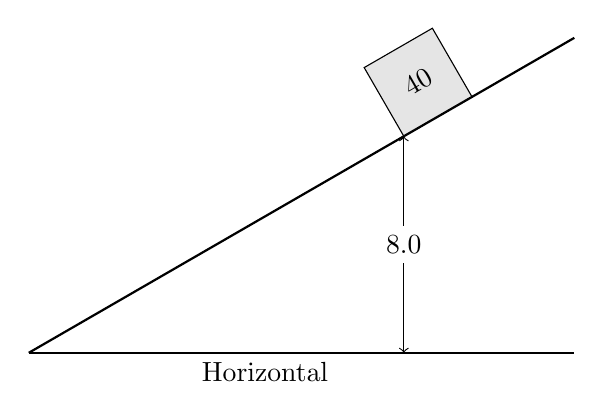
\begin{tikzpicture}
        %% Plane
        \draw[thick] (0,0) -- (30:8);
        %\draw[thick] (0,0) -- (5.20,0);
        \draw[thick] (0,0) -- (6.93,0);
        \node[anchor=north] at (3,0) {Horizontal};
        %% Mass
        \node[anchor=south,fill=white!90!black,rotate=30,draw,minimum size=1cm] at (30:6) {\SI{40}{\newton}};
        %% distance
        \draw[<->] (30:5.5) -- ++(270:2.75) node[pos=0.5,anchor=center,fill=white] {\SI{8.0}{\meter}};
    \end{tikzpicture}
    \end{center}
    If \SI{50}{\joule} of heat is generated as the block slides down the incline,
        the maximum kinetic energy of the block at the bottom of the incline is:
    \begin{multicols}{2}
    \begin{choices}
        \wrongchoice{\SI{50}{\joule}}
      \correctchoice{\SI{270}{\joule}}
        \wrongchoice{\SI{320}{\joule}}
        \wrongchoice{\SI{3100}{\joule}}
    \end{choices}
    \end{multicols}
\end{question}
}

\element{nysed}{
\begin{question}{Jan2008-Q36}
    A joule (\si{\joule}) is equivalent to a:
    \begin{choices}
      \correctchoice{newton meter (\si{\newton\meter})}
        \wrongchoice{newton second (\si{\newton\second})}
        \wrongchoice{newton per meter (\si{\newton\per\meter})}
        \wrongchoice{newton per second (\si{\newton\per\second})}
    \end{choices}
\end{question}
}

\element{nysed}{
\begin{question}{Jan2008-Q41}
    Which graph best represents the relationship between the elastic potential energy stored in a spring and its elongation from equilibrium?
    \begin{multicols}{2}
    \begin{choices}
        \AMCboxDimensions{down=-2.5em}
        \correctchoice{
            \begin{tikzpicture}
                \begin{axis}[
                    axis y line=left,
                    axis x line=bottom,
                    axis line style={->},
                    xlabel={elongation},
                    xtick=\empty,
                    ylabel={potential energy},
                    ytick=\empty,
                    xmin=0,xmax=11,
                    ymin=0,ymax=11,
                    width=\columnwidth,
                    very thin,
                ]
                \addplot[line width=1pt,domain=0:10]{0.1*x*x};
                \end{axis}
            \end{tikzpicture}
        }
        \wrongchoice{
            \begin{tikzpicture}
                \begin{axis}[
                    axis y line=left,
                    axis x line=bottom,
                    axis line style={->},
                    xlabel={elongation},
                    xtick=\empty,
                    ylabel={potential energy},
                    ytick=\empty,
                    xmin=0,xmax=11,
                    ymin=0,ymax=11,
                    width=\columnwidth,
                    very thin,
                ]
                \addplot[line width=1pt,domain=0:10]{8};
                \end{axis}
            \end{tikzpicture}
        }
        \wrongchoice{
            \begin{tikzpicture}
                \begin{axis}[
                    axis y line=left,
                    axis x line=bottom,
                    axis line style={->},
                    xlabel={elongation},
                    xtick=\empty,
                    ylabel={potential energy},
                    ytick=\empty,
                    xmin=0,xmax=11,
                    ymin=0,ymax=11,
                    width=\columnwidth,
                    very thin,
                ]
                \addplot[line width=1pt,domain=0:10]{10/x};
                \end{axis}
            \end{tikzpicture}
        }
        \wrongchoice{
            \begin{tikzpicture}
                \begin{axis}[
                    axis y line=left,
                    axis x line=bottom,
                    axis line style={->},
                    xlabel={elongation},
                    xtick=\empty,
                    ylabel={potential energy},
                    ytick=\empty,
                    xmin=0,xmax=11,
                    ymin=0,ymax=11,
                    width=\columnwidth,
                    very thin,
                ]
                \addplot[line width=1pt,domain=0:10]{x};
                \end{axis}
            \end{tikzpicture}
        }
    \end{choices}
    \end{multicols}
\end{question}
}


%% Section June2007
%%--------------------
\element{nysed}{
\begin{question}{June2007-Q11}
    The table below lists the mass and speed of each of four objects.
    \begin{center}
    \begin{tabular}{ccc}
        \toprule
        Objects & Mass (\si{\kilo\gram}) & Speed (\si{\meter\per\second}) \\
        \midrule
        A   & 1.0   & 4.0 \\
        B   & 2.0   & 2.0 \\
        C   & 0.5   & 4.0 \\
        D   & 4.0   & 1.0 \\
        \bottomrule
    \end{tabular}
    \end{center}
    %% NOTE: TODO: questionmult and table in options ??
    Which two objects have the same kinetic energy?
    \begin{multicols}{2}
    \begin{choices}
      \correctchoice{$B$ and $C$}
        \wrongchoice{$A$ and $D$}
        \wrongchoice{$B$ and $D$}
        \wrongchoice{$A$ and $C$}
    \end{choices}
    \end{multicols}
\end{question}
}

\element{nysed}{
\begin{question}{June2007-Q43}
    A pendulum is pulled to the side and released from rest.
    Which graph best represents the relationship between the gravitational potential energy of the pendulum and its displacement from its point of release?
    \begin{multicols}{2}
    \begin{choices}
        \AMCboxDimensions{down=-2.5em}
        \correctchoice{
            \begin{tikzpicture}
                \begin{axis}[
                    axis y line=left,
                    axis x line=bottom,
                    axis line style={->},
                    xlabel={displacement},
                    xtick=\empty,
                    ylabel={potential energy},
                    ytick=\empty,
                    xmin=0,xmax=11,
                    ymin=0,ymax=11,
                    width=\columnwidth,
                    very thin,
                ]
                \addplot[line width=1pt,domain=0:10]{0.4 * (x-5)*(x-5)};
                \end{axis}
            \end{tikzpicture}
        }
        \wrongchoice{
            \begin{tikzpicture}
                \begin{axis}[
                    axis y line=left,
                    axis x line=bottom,
                    axis line style={->},
                    xlabel={displacement},
                    xtick=\empty,
                    ylabel={potential energy},
                    ytick=\empty,
                    xmin=0,xmax=11,
                    ymin=0,ymax=11,
                    width=\columnwidth,
                    very thin,
                ]
                \addplot[line width=1pt,domain=0:10]{10 - 0.4*(x-5)*(x-5)};
                \end{axis}
            \end{tikzpicture}
        }
        \wrongchoice{
            \begin{tikzpicture}
                \begin{axis}[
                    axis y line=left,
                    axis x line=bottom,
                    axis line style={->},
                    xlabel={displacement},
                    xtick=\empty,
                    ylabel={potential energy},
                    ytick=\empty,
                    xmin=0,xmax=11,
                    ymin=0,ymax=11,
                    width=\columnwidth,
                    very thin,
                ]
                \addplot[line width=1pt,domain=0:10]{8};
                \end{axis}
            \end{tikzpicture}
        }
        \wrongchoice{
            \begin{tikzpicture}
                \begin{axis}[
                    axis y line=left,
                    axis x line=bottom,
                    axis line style={->},
                    xlabel={displacement},
                    xtick=\empty,
                    ylabel={potential energy},
                    ytick=\empty,
                    xmin=0,xmax=11,
                    ymin=0,ymax=11,
                    width=\columnwidth,
                    very thin,
                ]
                \addplot[line width=1pt,domain=0:10]{x};
                \end{axis}
            \end{tikzpicture}
        }
    \end{choices}
    \end{multicols}
\end{question}
}


%% Section Jan2007
%%--------------------
\element{nysed}{
\begin{question}{Jan2007-Q12}
    A spring with spring constant of \SI{80}{\newton\per\meter} is displaced \SI{0.30}{\meter} from its equilibrium position.
    The potential energy stored in the spring is:
    \begin{multicols}{2}
    \begin{choices}
      \correctchoice{\SI{3.6}{\joule}}
        \wrongchoice{\SI{7.2}{\joule}}
        \wrongchoice{\SI{12}{\joule}}
        \wrongchoice{\SI{24}{\joule}}
    \end{choices}
    \end{multicols}
\end{question}
}

\element{nysed}{
\begin{question}{Jan2007-Q13}
    The work done in accelerating an object along a frictionless horizontal surface is equal to the change in the object's:
    \begin{multicols}{2}
    \begin{choices}
      \correctchoice{kinetic energy}
        \wrongchoice{potential energy}
        \wrongchoice{momentum}
        \wrongchoice{velocity}
    \end{choices}
    \end{multicols}
\end{question}
}

\element{nysed}{
\begin{question}{Jan2007-Q14}
    As a block slides across a table, its speed decreases while its temperature increases.
    Which two changes occur in the block's energy as it slides?
    \begin{choices}
      \correctchoice{a decrease in kinetic energy and an increase in internal energy}
        \wrongchoice{a increase in kinetic energy and an decrease in internal energy}
        \wrongchoice{a decrease in both kinetic energy and internal energy}
        \wrongchoice{a increase in both kinetic energy and internal energy}
    \end{choices}
\end{question}
}

%% NOTE: possible duplicate?
\element{nysed}{
\begin{question}{Jan2007-Q40}
    Which graph best represents the relationship between the gravitational potential energy of an object near the surface of Earth and its height above Earth's surface?
    \begin{multicols}{2}
    \begin{choices}
        \AMCboxDimensions{down=-2.5em}
        \correctchoice{
            \begin{tikzpicture}
                \begin{axis}[
                    axis y line=left,
                    axis x line=bottom,
                    axis line style={->},
                    xlabel={height},
                    xtick=\empty,
                    ylabel={potential energy},
                    ytick=\empty,
                    xmin=0,xmax=10.5,
                    ymin=0.0,ymax=10.5,
                    width=0.98\columnwidth,
                    very thin,
                ]
                \addplot[line width=1pt,domain=0:10]{x};
                \end{axis}
            \end{tikzpicture}
        }
        \wrongchoice{
            \begin{tikzpicture}
                \begin{axis}[
                    axis y line=left,
                    axis x line=bottom,
                    axis line style={->},
                    xlabel={height},
                    xtick=\empty,
                    ylabel={potential energy},
                    ytick=\empty,
                    xmin=0,xmax=10.5,
                    ymin=0.0,ymax=10.5,
                    width=0.98\columnwidth,
                    very thin,
                ]
                \addplot[line width=1pt,domain=0:10]{8};
                \end{axis}
            \end{tikzpicture}
        }
        \wrongchoice{
            \begin{tikzpicture}
                \begin{axis}[
                    axis y line=left,
                    axis x line=bottom,
                    axis line style={->},
                    xlabel={height},
                    xtick=\empty,
                    ylabel={potential energy},
                    ytick=\empty,
                    xmin=0,xmax=10.5,
                    ymin=0.0,ymax=10.5,
                    width=0.98\columnwidth,
                    very thin,
                ]
                \addplot[line width=1pt,domain=0:10]{10/x};
                \end{axis}
            \end{tikzpicture}
        }
        \wrongchoice{
            \begin{tikzpicture}
                \begin{axis}[
                    axis y line=left,
                    axis x line=bottom,
                    axis line style={->},
                    xlabel={height},
                    xtick=\empty,
                    ylabel={potential energy},
                    ytick=\empty,
                    xmin=0,xmax=10.5,
                    ymin=0.0,ymax=10.5,
                    width=0.98\columnwidth,
                    very thin,
                ]
                \addplot[line width=1pt,domain=0:10]{10-x};
                \end{axis}
            \end{tikzpicture}
        }
    \end{choices}
    \end{multicols}
\end{question}
}

\element{nysed}{
\begin{question}{Jan2007-Q44}
    A \SI{1.00}{\kilo\gram} ball is dropped from the top of a building.
    Just before striking the ground, the ball's speed is \SI{12.0}{\meter\per\second}.
    What was the ball's gravitational potential energy,
        relative to the ground,
        at the instant it was dropped?
    [Neglect friction.]
    \begin{multicols}{2}
    \begin{choices}
        \wrongchoice{\SI{6.00}{\joule}}
        \wrongchoice{\SI{24.0}{\joule}}
      \correctchoice{\SI{72.0}{\joule}}
        \wrongchoice{\SI{144}{\joule}}
    \end{choices}
    \end{multicols}
\end{question}
}


\element{nysed}{
\begin{question}{Jan2007-Q45}
    As shown in the diagram below, a child applies a constant \SI{20}{\newton} force along the handle of a wagon which makes a \ang{25} angle with the horizontal.
    \begin{center}
        %% NOTE: TODO: draw tikz, borrow from halliday pulley
        %% NOTE: human is not necessary, just arbitray vector
        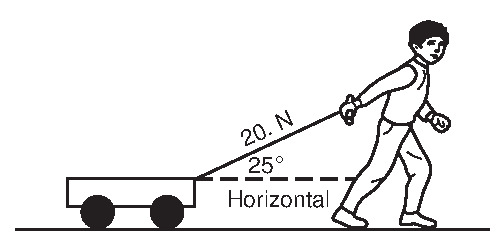
\includegraphics[keepaspectratio,scale=1.0]{Jan2007-Q45}
    \end{center}
    How much work does the child do in moving the wagon a horizontal distance of \SI{4.0}{\meter}?
    \begin{multicols}{2}
    \begin{choices}
      \correctchoice{\SI{73}{\joule}}
        \wrongchoice{\SI{5.0}{\joule}}
        \wrongchoice{\SI{80}{\joule}}
        \wrongchoice{\SI{34}{\joule}}
    \end{choices}
    \end{multicols}
\end{question}
}


%% Section June2006
%%--------------------
\element{nysed}{
\begin{question}{June2006-Q12}
    A \SI{2.0}{\kilo\gram} block sliding down a ramp from a height of \SI{3.0}{\meter} above the ground reaches the ground with a kinetic energy of \SI{50}{\joule}.
    The total work done by friction on the blocks as it slides down the ramp is approximately:
    \begin{multicols}{2}
    \begin{choices}
      \correctchoice{\SI{9}{\joule}}
        \wrongchoice{\SI{6}{\joule}}
        \wrongchoice{\SI{18}{\joule}}
        \wrongchoice{\SI{44}{\joule}}
    \end{choices}
    \end{multicols}
\end{question}
}

\element{nysed}{
\begin{question}{June2006-Q13}
    A person weighing \SI{6.0e2}{\newton} rides an elevator upward at an average speed of \SI{3.0}{\meter\per\second} for \SI{5.0}{\second}.
    How much does this person's gravitational potential energy increase as a result of this ride?
    \begin{multicols}{2}
    \begin{choices}
      \correctchoice{\SI{9e3}{\joule}}
        \wrongchoice{\SI{3e3}{\joule}}
        \wrongchoice{\SI{3.6e2}{\joule}}
        \wrongchoice{\SI{1.8e3}{\joule}}
    \end{choices}
    \end{multicols}
\end{question}
}

\element{nysed}{
\begin{question}{June2006-Q16}
    During an emergency stop, a \SI{1.5e3}{\kilo\gram} car lost a total of \SI{2.0e5}{\joule} of kinetic energy.
    What was the speed of the car at the moment the brakes were applied?
    \begin{multicols}{2}
    \begin{choices}
      \correctchoice{\SI{20}{\meter\per\second}}
        \wrongchoice{\SI{25}{\meter\per\second}}
        \wrongchoice{\SI{10.}{\meter\per\second}}
        \wrongchoice{\SI{14}{\meter\per\second}}
    \end{choices}
    \end{multicols}
\end{question}
}

\element{nysed}{
\begin{question}{June2006-Q41}
    Which two quantities can be expressed using same units?
    \begin{choices}
      \correctchoice{impulse and momentum}
        \wrongchoice{energy and force}
        \wrongchoice{impulse and force}
        \wrongchoice{momentum and energy}
    \end{choices}
\end{question}
}

\element{nysed}{
\begin{question}{June2006-Q45}
    A box is pushed to the right with a varying horizontal force.
    The graph below represents the relationship between the applied force and the distance the box moves.
    \begin{center}
    \begin{tikzpicture}
        \begin{axis}[
            axis y line=left,
            axis x line=bottom,
            axis line style={->},
            xlabel={distance},
            x unit=\si{\meter},
            xtick={0,3,6},
            ylabel={force},
            y unit=\si{\newton},
            ytick={0,3,6,9},
            xmin=0,xmax=6.5,
            ymin=0,ymax=6.5,
            grid=major,
            width=0.8\columnwidth,
            height=0.5\columnwidth,
            very thin,
        ]
        \addplot[line width=1pt,domain=0:3]{6};
        \addplot[line width=1pt,domain=3:6]{6 - 2*(x-3)};
        \end{axis}
    \end{tikzpicture}
    \end{center}
    What is the total work done in moving the box \SI{6.0}{\meter}?
    \begin{multicols}{2}
    \begin{choices}
      \correctchoice{\SI{27}{\joule}}
        \wrongchoice{\SI{36}{\joule}}
        \wrongchoice{\SI{9.0}{\joule}}
        \wrongchoice{\SI{18}{\joule}}
    \end{choices}
    \end{multicols}
\end{question}
}


%% Section Jan2006
%%--------------------
\element{nysed}{
\begin{question}{Jan2006-Q15}
    A \SI{6.8}{\kilo\gram} block is sliding down a horizontal,
        frictionless surface at a constant speed of \SI{6.0}{\meter\per\second}.
    The kinetic energy of the block is approximately:
    \begin{multicols}{2}
    \begin{choices}
      \correctchoice{\SI{120}{\joule}}
        \wrongchoice{\SI{20}{\joule}}
        \wrongchoice{\SI{41}{\joule}}
        \wrongchoice{\SI{240}{\joule}}
    \end{choices}
    \end{multicols}
\end{question}
}

\element{nysed}{
\begin{question}{Jan2006-Q16}
    Through what vertical distance is a \SI{50}{\newton} object moved if \SI{250}{\joule} of work is done against the gravitational field of Earth?
    \begin{multicols}{2}
    \begin{choices}
      \correctchoice{\SI{5.0}{\meter}}
        \wrongchoice{\SI{2.5}{\meter}}
        \wrongchoice{\SI{9.8}{\meter}}
        \wrongchoice{\SI{25}{\meter}}
    \end{choices}
    \end{multicols}
\end{question}
}

\element{nysed}{
\begin{question}{Jan2006-Q17}
    When a mass is placed on a spring with a spring constant of \SI{15}{\newton\per\meter},
        the spring is compressed \SI{0.25}{\meter}.
    How much elastic potential energy is stored in the spring?
    \begin{multicols}{2}
    \begin{choices}
      \correctchoice{\SI{0.47}{\joule}}
        \wrongchoice{\SI{0.94}{\joule}}
        \wrongchoice{\SI{1.9}{\joule}}
        \wrongchoice{\SI{3.8}{\joule}}
    \end{choices}
    \end{multicols}
\end{question}
}

\element{nysed}{
\begin{question}{Jan2006-Q18}
    Two students of equal weight go from the first floor to the second floor.
    The first student uses an elevator and the second student walks up a flight of stairs.
    compared to the gravitational potential energy gained by the first student,
        the gravitational potential energy gained by the second student is:
    \begin{multicols}{3}
    \begin{choices}
      \correctchoice{the same}
        \wrongchoice{less}
        \wrongchoice{greater}
    \end{choices}
    \end{multicols}
\end{question}
}

\element{nysed}{
\begin{question}{Jan2006-Q44}
    An object falls freely near Earth's surface.
    Which graph best represents the relationship between the object's kinetic energy and its time of fall?
    \begin{multicols}{2}
    \begin{choices}
        \AMCboxDimensions{down=-2.5em}
        \correctchoice{
            \begin{tikzpicture}
                \begin{axis}[
                    axis y line=left,
                    axis x line=bottom,
                    axis line style={->},
                    xlabel={time},
                    xtick=\empty,
                    ylabel={kinetic energy},
                    ytick=\empty,
                    xmin=0,xmax=10.5,
                    ymin=0.0,ymax=10.5,
                    width=0.98\columnwidth,
                    very thin,
                ]
                \addplot[line width=1pt,domain=0:10]{0.1*x*x};
                \end{axis}
            \end{tikzpicture}
        }
        \wrongchoice{
            \begin{tikzpicture}
                \begin{axis}[
                    axis y line=left,
                    axis x line=bottom,
                    axis line style={->},
                    xlabel={time},
                    xtick=\empty,
                    ylabel={kinetic energy},
                    ytick=\empty,
                    xmin=0,xmax=10.5,
                    ymin=0.0,ymax=10.5,
                    width=0.98\columnwidth,
                    very thin,
                ]
                \addplot[line width=1pt,domain=0:10]{x};
                \end{axis}
            \end{tikzpicture}
        }
        \wrongchoice{
            \begin{tikzpicture}
                \begin{axis}[
                    axis y line=left,
                    axis x line=bottom,
                    axis line style={->},
                    xlabel={time},
                    xtick=\empty,
                    ylabel={kinetic energy},
                    ytick=\empty,
                    xmin=0,xmax=10.5,
                    ymin=0.0,ymax=10.5,
                    width=0.98\columnwidth,
                    very thin,
                ]
                \addplot[line width=1pt,domain=0:10]{10-x};
                \end{axis}
            \end{tikzpicture}
        }
        \wrongchoice{
            \begin{tikzpicture}
                \begin{axis}[
                    axis y line=left,
                    axis x line=bottom,
                    axis line style={->},
                    xlabel={time},
                    xtick=\empty,
                    ylabel={kinetic energy},
                    ytick=\empty,
                    xmin=0,xmax=10.5,
                    ymin=0.0,ymax=10.5,
                    width=0.98\columnwidth,
                    very thin,
                ]
                \addplot[line width=1pt,domain=0:10]{10-0.1*x*x};
                \end{axis}
            \end{tikzpicture}
        }
    \end{choices}
    \end{multicols}
\end{question}
}


%% Section June2005
%%--------------------
\element{nysed}{
\begin{question}{June2005-Q16}
    As shown in the diagram below,
        a student exerts an average force of \SI{600}{\newton} on a rope to lift a \SI{50}{\kilo\gram} crate a vertical distance of \SI{3.00}{\meter}.
    \begin{center}
        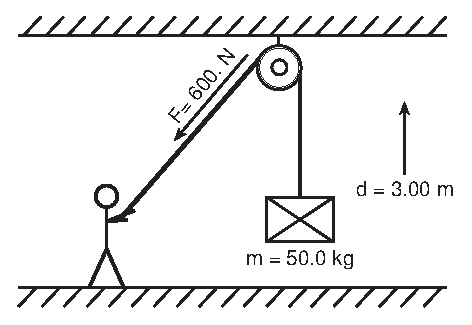
\includegraphics[keepaspectratio,scale=0.75]{June2005-Q16}
    \end{center}
    Compared to the work done by the student,
        the gravitational potential energy gained by the crate is:
    \begin{choices}
      \correctchoice{exactly the same}
        \wrongchoice{\SI{330}{\joule} less}
        \wrongchoice{\SI{330}{\joule} more}
        \wrongchoice{\SI{150}{\joule} more}
    \end{choices}
\end{question}
}

\element{nysed}{
\begin{question}{June2005-Q17}
    A \SI{1.0}{\kilo\gram} book resting on the ground is moved \SI{1.0}{\meter} at various angles relative to the horizontal.
    In which direction does the \SI{1.0}{\meter} displacement produce the greatest increase in the book's gravitational potential energy?
    \begin{multicols}{2}
    \begin{choices}\footnotesize
        \AMCboxDimensions{down=-0.7cm}
        \correctchoice{
            \begin{tikzpicture}
                %% Book
                \draw[white] (-1.5,0) rectangle (1.5,2);
                \node[draw,rectangle,minimum size=1.00cm,anchor=center]
                    (B) at (-0.5,0.5) {Book};
                %% Vector
                \draw[thick,->] (B.north) -- ++(90:1) node[pos=0.0,anchor=south west] {\ang{90}};
                %% Floor
                \draw[thick] (-1.5,0) -- (1.5,0);
                \node[anchor=north,pattern=north east lines,minimum width=3cm] at (0,0) {};
                \node[anchor=north] at (-0.5,-1em) {Ground};
            \end{tikzpicture}
        }
        \wrongchoice{
            \begin{tikzpicture}
                %% Book
                \draw[white] (-1.5,0) rectangle (1.5,2);
                \node[draw,rectangle,minimum size=1.00cm,anchor=center]
                    (B) at (-0.5,0.5) {Book};
                %% Vector
                \draw[thick,->] (B.north east) -- ++(45:1);
                \draw[thick,dotted,<->] (1.0,0) arc (0:45:2.0) node[pos=0.5,anchor=west] {\ang{45}};
                %% Floor
                \draw[thick] (-1.5,0) -- (1.5,0);
                \node[anchor=north,pattern=north east lines,minimum width=3cm] at (0,0) {};
                \node[anchor=north] at (-0.5,-1em) {Ground};
            \end{tikzpicture}
        }
        \wrongchoice{
            \begin{tikzpicture}
                %% Book
                \draw[white] (-1.5,0) rectangle (1.5,2);
                \node[draw,rectangle,minimum size=1.00cm,anchor=center]
                    (B) at (-0.5,0.5) {Book};
                %% Vector
                \draw[thick,->] (B.east) -- ++(20:1);
                \draw[thick,dotted,<->] (0.66,0) arc (0:20:2.04) node[pos=0.5,anchor=west] {\ang{20}};
                %% Floor
                \draw[thick] (-1.5,0) -- (1.5,0);
                \node[anchor=north,pattern=north east lines,minimum width=3cm] at (0,0) {};
                \node[anchor=north] at (-0.5,-1em) {Ground};
            \end{tikzpicture}
        }
        \wrongchoice{
            \begin{tikzpicture}
                %% Book
                \draw[white] (-1.5,0) rectangle (1.5,2);
                \node[draw,rectangle,minimum size=1.00cm,anchor=center]
                    (B) at (-0.5,0.5) {Book};
                %% Vector
                \draw[->] (B.east) -- ++(0:1) node[pos=0.0,anchor=south west] {\ang{0}};
                %% Floor
                \draw[thick] (-1.5,0) -- (1.5,0);
                \node[anchor=north,pattern=north east lines,minimum width=3cm] at (0,0) {};
                \node[anchor=north] at (-0.5,-1em) {Ground};
            \end{tikzpicture}
        }
    \end{choices}
    \end{multicols}
\end{question}
}


%% Section Jan2005
%%--------------------
\element{nysed}{
\begin{question}{Jan2005-Q20}
    What is the gravitational energy with respect to the surface of the water of a \SI{75.0}{\kilo\gram} diver located \SI{3.00}{\meter} above the water?
    \begin{multicols}{2}
    \begin{choices}
      \correctchoice{\SI{2.21e3}{\joule}}
        \wrongchoice{\SI{2.17e4}{\joule}}
        \wrongchoice{\SI{2.25e2}{\joule}}
        \wrongchoice{\SI{2.29e1}{\joule}}
    \end{choices}
    \end{multicols}
\end{question}
}

\element{nysed}{
\begin{question}{Jan2005-Q21}
    A \SI{60.0}{\kilo\gram} runner has \SI{1920}{\joule} of kinetic energy.
    At what speed is she running?
    \begin{multicols}{2}
    \begin{choices}
      \correctchoice{\SI{8.00}{\meter\per\second}}
        \wrongchoice{\SI{5.66}{\meter\per\second}}
        \wrongchoice{\SI{32.0}{\meter\per\second}}
        \wrongchoice{\SI{64.0}{\meter\per\second}}
    \end{choices}
    \end{multicols}
\end{question}
}

\element{nysed}{
\begin{question}{Jan2005-Q22}
    The diagram below shows points $A$, $B$, and $C$ at or near the Earth's surface.
    As a mass is moved from $A$ to $B$, \SI{100}{\joule} of work are done against gravity.
    \begin{center}
    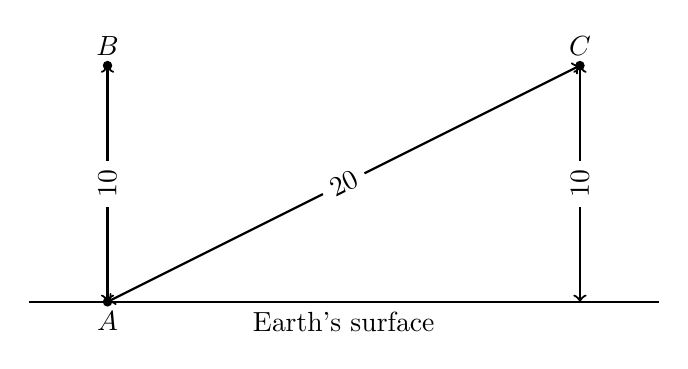
\begin{tikzpicture}
        %% Earth's surface
        \draw[thick] (-4,0) -- (4,0) node[pos=0.5,anchor=north] {Earth's surface};
        %% Point A, B, C
        \draw[fill] (-3,0) circle (1.5pt) node[anchor=north] {$A$};
        \draw[fill] (-3,3) circle (1.5pt) node[anchor=south] {$B$};
        \draw[fill] (+3,3) circle (1.5pt) node[anchor=south] {$C$};
        %% 10 meter labels
        \draw[thick,<->] (-3,0) -- (-3,3) node[pos=0.5,anchor=center,rotate=90,fill=white] {\SI{10}{\meter}};
        \draw[thick,<->] (+3,0) -- (+3,3) node[pos=0.5,anchor=center,rotate=90,fill=white] {\SI{10}{\meter}};
        %% 20 meter labels
        \draw[thick,<->] (-3,0) -- (+3,3) node[pos=0.5,anchor=center,rotate=26.6,fill=white] {\SI{20}{\meter}};
    \end{tikzpicture}
    \end{center}
    What is the amount of work done against gravity as an identical mass is moved from $A$ to $C$?
    \begin{multicols}{2}
    \begin{choices}
      \correctchoice{\SI{100}{\joule}}
        \wrongchoice{\SI{200}{\joule}}
        \wrongchoice{\SI{173}{\joule}}
        \wrongchoice{\SI{273}{\joule}}
    \end{choices}
    \end{multicols}
\end{question}
}

\element{nysed}{
\begin{question}{Jan2005-Q23}
    When a force moves an object over a rough,
        horizontal surface at constant velocity,
        the work done against friction produces an increase in the object's:
    \begin{multicols}{2}
    \begin{choices}
      \correctchoice{internal energy}
        \wrongchoice{weight}
        \wrongchoice{potential energy}
        \wrongchoice{internal energy}
    \end{choices}
    \end{multicols}
\end{question}
}


%% Section June2004
%%--------------------
\element{nysed}{
\begin{question}{June2004-Q11}
    The work done in moving a block across a rough surface and the heat energy gained by the block can both be measured in:
    \begin{multicols}{2}
    \begin{choices}
      \correctchoice{joules}
        \wrongchoice{degrees}
        \wrongchoice{newtons}
        \wrongchoice{watts}
    \end{choices}
    \end{multicols}
\end{question}
}

\element{nysed}{
\begin{question}{June2004-Q12}
    Two weightlifters, one \SI{1.5}{\meter} tall and one \SI{2.0}{\meter} tall,
        raise identical \SI{50}{\kilo\gram} masses above their heads.
    Compared to the work done by the weightlifter who is \SI{1.5}{\meter} tall,
        the work done by the weightlifter who is \SI{2.0}{\meter} tall is:
    \begin{multicols}{3}
    \begin{choices}
      \correctchoice{greater}
        \wrongchoice{less}
        \wrongchoice{the same}
    \end{choices}
    \end{multicols}
\end{question}
}

\element{nysed}{
\begin{question}{June2004-Q13}
    A \SI{45}{\kilo\gram} boy is riding a \SI{15}{\kilo\gram} bicycle with a speed of \SI{8.00}{\meter\per\second}.
    What is the combined kinetic energy of the boy and the bicycle?
    \begin{multicols}{2}
    \begin{choices}
      \correctchoice{\SI{1920}{\joule}}
        \wrongchoice{\SI{1440}{\joule}}
        \wrongchoice{\SI{480}{\joule}}
        \wrongchoice{\SI{240}{\joule}}
    \end{choices}
    \end{multicols}
\end{question}
}


%% Section Jan2004
%%--------------------
\element{nysed}{
\begin{question}{Jan2004-Q18}
    A student does \SI{60}{\joule} of work pushing a \SI{3.0}{\kilo\gram} box up the full length of a ramp that is \SI{5.0}{\meter} long.
    What is the magnitude of the force applied to the box to do this work?
    \begin{multicols}{2}
    \begin{choices}
      \correctchoice{\SI{12}{\newton}}
        \wrongchoice{\SI{15}{\newton}}
        \wrongchoice{\SI{4.0}{\newton}}
        \wrongchoice{\SI{20.}{\newton}}
    \end{choices}
    \end{multicols}
\end{question}
}


%% Section June2003
%%--------------------
\element{nysed}{
\begin{question}{June2003-Q01}
    The diagram below shows a \SI{40}{\kilo\gram} crate on a frictionless plane at angle $\theta$ to the horizontal.
    The crate is pushed at constant speed up the incline from point $A$ to point $B$ by force $F$.
    \begin{center}
    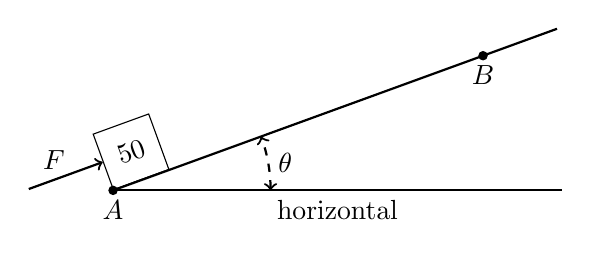
\begin{tikzpicture}
        %% Ramp
        \draw[thick] (0,0) -- (20:6);
        %% A and B Label
        \draw[fill] (20:0) circle  (1.5pt)
            node[anchor=north] {$A$};
        \draw[fill] (20:5) circle  (1.5pt)
            node[anchor=north] {$B$};
        %% Theta label
        \draw[thick,<->,dashed] (0:2) arc (0:20:2)
            node[pos=0.5,anchor=west] {$\theta$};
        %% Block
        \node[draw,rectangle,minimum size=0.75cm,rotate=20,anchor=south west]
            (B) at (20:0) {\SI{50}{\kilo\gram}};
        \draw[thick,<-] (B.west) -- ++ (200:1)
            node[pos=0.66,anchor=south] {$F$};
        %% Horizontal
        \draw[thick] (0:0) -- (0:5.7)
            node[pos=0.5,anchor=north] {horizontal};
    \end{tikzpicture}
    \end{center}
    If angle $\theta$ were increased, what would be the effect on the magnitude of force $F$ and the total work $W$ done on the create as it is moved from $A$ to $B$.
    The worker's pull on the handle of the cart can best be described as a force having:
    \begin{choices}
      \correctchoice{$W$ would increase and the magnitude of $F$ would increase.}
        \wrongchoice{$W$ would remain the same and the magnitude of $F$ would decrease.}
        \wrongchoice{$W$ would remain the same and the magnitude of $F$ would increase.}
        \wrongchoice{$W$ would increase and the magnitude of $F$ would decrease.}
    \end{choices}
\end{question}
}

\element{nysed}{
\begin{question}{June2003-Q10}
    A \SI{10}{\newton} force is required to hold a stretched spring \SI{0.20}{\meter} from its rest position.
    What is the potential energy stored in the stretched spring?
    \begin{multicols}{2}
    \begin{choices}
      \correctchoice{\SI{1.0}{\joule}}
        \wrongchoice{\SI{2.0}{\joule}}
        \wrongchoice{\SI{5.0}{\joule}}
        \wrongchoice{\SI{50}{\joule}}
    \end{choices}
    \end{multicols}
\end{question}
}


%% Section Jan2003
%%--------------------
\element{nysed}{
\begin{question}{Jan2003-Q12}
    The amount of work done against friction to slide a box in a straight line across a uniform,
        horizontal floor depends most on the:
    \begin{choices}
      \correctchoice{distance taken to move the box}
        \wrongchoice{time taken to move the box}
        \wrongchoice{speed of the box}
        \wrongchoice{direction of the box's motion}
    \end{choices}
\end{question}
}

\element{nysed}{
\begin{question}{Jan2003-Q13}
    A \SI{1.2}{\kilo\gram} block and a \SI{1.8}{\kilo\gram} block are initially at rest on a frictionless, horizontal surface.
    When a compressed spring between the blocks is released,
        the \SI{1.8}{\kilo\gram} block moves to the right at \SI{2.0}{\meter\per\second} as shown.
    \begin{center}
    \begin{tikzpicture}
        %% Floor
        \draw (-4,0) -- (4,0);
        \node[anchor=north,fill,pattern=north east lines,minimum width=8cm, minimum height=0.05cm] at (0,0) {};
        \node[anchor=north] at (0,-0.25) {Frictionless horizontal surface};
        %% blocks
        \node[anchor=south,draw,minimum size=1.5cm,fill=white!90!black] (L) at (-2,0) {\SI{1.2}{\kilo\gram}};
        \node[anchor=south,draw,minimum size=1.5cm,fill=white!90!black] (R) at (+2,0) {\SI{1.8}{\kilo\gram}};
        %% velocity
        \draw[thick,->] (L.north east) ++(90:0.5) -- ++(180:1.5cm) node[pos=0.5,anchor=south] {?};
        \draw[thick,->] (R.north west) ++(90:0.5) -- ++(0:1.5cm) node[pos=0.5,anchor=south] {\SI{2.0}{\meter\per\second}};
        %% Spring
        \draw[thick,decoration={aspect=0.2,segment length=2mm,amplitude=4mm,coil},decorate] (L.east) -- (R.west);
    \end{tikzpicture}
    \end{center}
    What is the speed of the \SI{1.2}{\kilo\gram} block after the spring is released?
    \begin{multicols}{2}
    \begin{choices}
      \correctchoice{\SI{3.0}{\meter\per\second}}
        \wrongchoice{\SI{1.4}{\meter\per\second}}
        \wrongchoice{\SI{2.0}{\meter\per\second}}
        \wrongchoice{\SI{3.6}{\meter\per\second}}
    \end{choices}
    \end{multicols}
\end{question}
}

\element{nysed}{
\begin{question}{Jan2003-Q15}
    An object weighs \SI{15}{\newton} is listed from the ground of \SI{0.22}{\meter}.
    The increase in the object's gravitational potential energy is approximately:
    \begin{multicols}{2}
    \begin{choices}
      \correctchoice{\SI{3.3}{\joule}}
        \wrongchoice{\SI{33}{\joule}}
        \wrongchoice{\SI{310}{\joule}}
        \wrongchoice{\SI{0.34}{\joule}}
    \end{choices}
    \end{multicols}
\end{question}
}

\element{nysed}{
\begin{question}{Jan2003-Q41}
    The spring of a toy car is wound by pushing the car backward with an average force of \SI{15}{\newton} through a distance of \SI{0.50}{\meter}.
    How much elastic potential energy is stored in the car's spring during this process?
    \begin{multicols}{2}
    \begin{choices}
      \correctchoice{\SI{7.5}{\joule}}
        \wrongchoice{\SI{1.9}{\joule}}
        \wrongchoice{\SI{30}{\joule}}
        \wrongchoice{\SI{56}{\joule}}
    \end{choices}
    \end{multicols}
\end{question}
}


%% Section Aug2002
%%--------------------
\element{nysed}{
\begin{question}{Aug2002-Q08}
    A block weighing \SI{15}{\newton} is pulled to the top of an incline that is \SI{0.20}{\meter} above the ground, as shown below.
    \begin{center}
    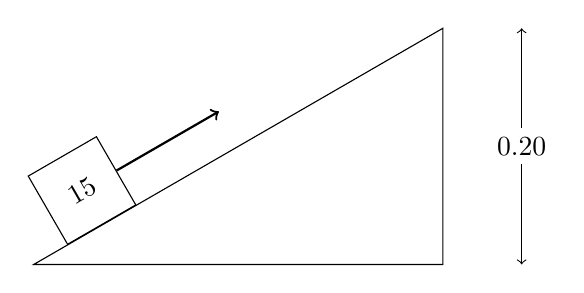
\begin{tikzpicture}
        %% plane
        \draw (0,0) -- (30:6) --++(270:3) -- cycle;
        %% block
        \node[anchor=south,rotate=30,draw,minimum size=1cm] (A) at (30:1) {\SI{15}{\newton}};
        %% force
        \draw[thick,->] (A.east) -- ++(30:1.5);
        %% height
        \draw[<->] (30:6) ++(0:1) -- ++(270:3) node[pos=0.5,anchor=center,fill=white] {\SI{0.20}{\meter}};
    \end{tikzpicture}
    \end{center}
    If \SI{4.0}{\joule} of work are needed to pull the block the full length of the incline,
        how much work is done against friction?
    \begin{multicols}{2}
    \begin{choices}
      \correctchoice{\SI{1.0}{\joule}}
        \wrongchoice{\SI{0.0}{\joule}}
        \wrongchoice{\SI{3.0}{\joule}}
        \wrongchoice{\SI{7.0}{\joule}}
    \end{choices}
    \end{multicols}
\end{question}
}

\element{nysed}{
\begin{question}{Aug2002-Q09}
    A \SI{1.0}{\kilo\gram} rubber ball traveling east at \SI{4.0}{\meter\per\second} hits a wall and bounces back toward the west at \SI{2.0}{\meter\per\second}.
    Compared to the kinetic energy of the ball before it hits the wall,
        the kinetic energy of the ball after it bounces off the wall is:
    \begin{choices}
      \correctchoice{one-fourth as great}
        \wrongchoice{one-half as great}
        \wrongchoice{the same}
        \wrongchoice{four times as great}
    \end{choices}
\end{question}
}

\element{nysed}{
\begin{question}{Aug2002-Q10}
    As a spring is stretched,
        its elastic potential energy:
    \begin{choices}
        \wrongchoice{decreases}
      \correctchoice{increases}
        \wrongchoice{remains the same}
    \end{choices}
\end{question}
}

\element{nysed}{
\begin{question}{Aug2002-Q12}
    A catapult with a spring constant of \SI{1.0e4}{\newton\per\meter} is required to launch an airplane from the deck of an aircraft carrier.
    The plane is released when it has been displaced \SI{0.50}{\meter} from its equilibrium position by the catapult.
    The energy acquired by the airplane from the catapult during takeoff is approximately:
    \begin{multicols}{2}
    \begin{choices}
      \correctchoice{\SI{1.3e3}{\joule}}
        \wrongchoice{\SI{2.0e4}{\joule}}
        \wrongchoice{\SI{2.5e3}{\joule}}
        \wrongchoice{\SI{1.0e4}{\joule}}
    \end{choices}
    \end{multicols}
\end{question}
}


%% Section June2002
%%--------------------
\element{nysed}{
\begin{question}{June2002-Q20}
    In the diagram below, \SI{400}{\joule} of work is done raising a \SI{72}{\newton} weight a vertical distance of \SI{5.0}{\meter}.
    \begin{center}
        %% NOTE: TODO: draw tikz
        %% NOTE: check cpo for pulley
        %% NOTE: this pulley is more involved.
        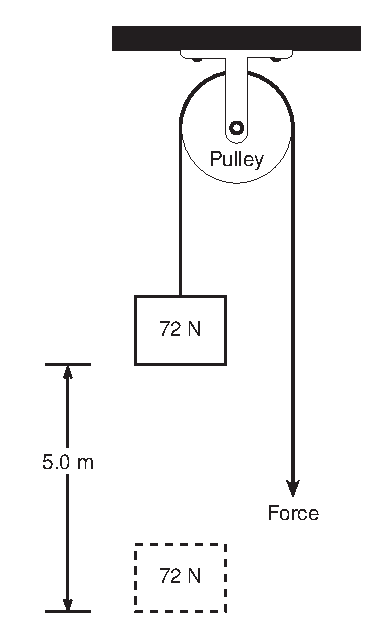
\includegraphics[keepaspectratio,scale=0.75]{June2002-Q20}
    \end{center}
    How much work is done to overcome friction as the weight is raised?
    \begin{multicols}{2}
    \begin{choices}
      \correctchoice{\SI{40}{\joule}}
        \wrongchoice{\SI{400}{\joule}}
        \wrongchoice{\SI{360}{\joule}}
        \wrongchoice{\SI{760}{\joule}}
    \end{choices}
    \end{multicols}
\end{question}
}

\element{nysed}{
\begin{question}{June2002-Q14}
    An object moving at a constant speed of \SI{25}{\meter\per\second} possesses \SI{450}{\joule} of kinetic energy.
    What is the object's mass?
    \begin{multicols}{2}
    \begin{choices}
        \wrongchoice{\SI{0.72}{\kilo\gram}}
      \correctchoice{\SI{1.4}{\kilo\gram}}
        \wrongchoice{\SI{18}{\kilo\gram}}
        \wrongchoice{\SI{36}{\kilo\gram}}
    \end{choices}
    \end{multicols}
\end{question}
}

\element{nysed}{
\begin{question}{June2002-Q15}
    The diagram below shows a moving,
        \SI{5.0}{\kilo\gram} cart at the foot of a hill, \SI{10.0}{\meter} high.
    \begin{center}
    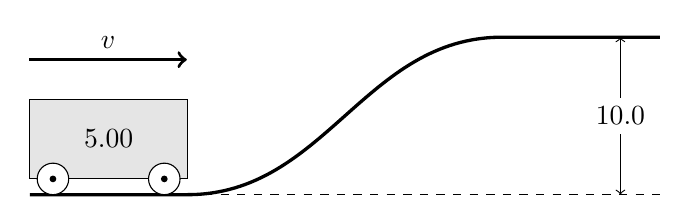
\begin{tikzpicture}
        %% Ground
        \draw[dashed] (-2,0) -- (4,0);
        \draw[very thick] (-4,0) -- (-2,0) to[out=0,in=180] (2,2) -- (4,2);
        \draw[<->] (3.5,0) -- (3.5,2) node[pos=0.5,anchor=center,fill=white] {\SI{10.0}{\meter}};
        %% Cart
        \node[draw,fill=white!90!black,minimum height=1.00cm,minimum width=2.00cm,anchor=south] (A) at (-3,0.2) {\SI{5.00}{\kilo\gram}};
        \draw[very thick,->] (A.north west) ++(90:0.5) -- ++(0:2cm) node[pos=0.5,anchor=south] {$v$};
        %% wheels
        \draw[fill=white] (A.south west) ++(0:0.3) circle (0.2);
        \draw[fill=black] (A.south west) ++(0:0.3) circle (1pt);
        \draw[fill=white] (A.south east) ++(180:0.3) circle (0.2);
        \draw[fill=black] (A.south east) ++(180:0.3) circle (1pt);
    \end{tikzpicture}
    \end{center}
    For the cart to reach the top of the hill,
        what is the minimum kinetic energy of the cart in the position shown?
    [Neglect energy loss due to friction]
    \begin{multicols}{2}
    \begin{choices}
        \wrongchoice{\SI{4.91}{\joule}}
        \wrongchoice{\SI{50.0}{\joule}}
      \correctchoice{\SI{250}{\joule}}
        \wrongchoice{\SI{491}{\joule}}
    \end{choices}
    \end{multicols}
\end{question}
}

\element{nysed}{
\begin{question}{June2002-Q16}
    A constant force of \SI{1900}{\newton} is required to keep an automobile having a mass of \SI{1.0e3}{\kilo\gram} moving at a constant speed of \SI{20}{\meter\per\second}.
    The work done in moving the automobile a distance of \SI{2.0e3}{\meter} is:
    \begin{multicols}{2}
    \begin{choices}
        \wrongchoice{\SI{2.0e4}{\joule}}
        \wrongchoice{\SI{3.8e4}{\joule}}
        \wrongchoice{\SI{2.0e6}{\joule}}
      \correctchoice{\SI{3.8e6}{\joule}}
    \end{choices}
    \end{multicols}
\end{question}
}

\element{nysed}{
\begin{question}{June2002-Q33}
    A spring of negligible mass has a spring constant of \SI{50}{\newton\per\meter}.
    If the spring is stretched \SI{0.40}{\meter} from its equilibrium position,
        how much potential energy is stored in the spring?
    \begin{multicols}{2}
    \begin{choices}
        \wrongchoice{\SI{20}{\joule}}
        \wrongchoice{\SI{10}{\joule}}
        \wrongchoice{\SI{8.0}{\joule}}
      \correctchoice{\SI{4.0}{\joule}}
    \end{choices}
    \end{multicols}
\end{question}
}

\element{nysed}{
\begin{question}{June2002-Q42}
    Which graph best represents the elastic potential energy stored in a spring as a function of its elongation?
    \begin{multicols}{2}
    \begin{choices}
        \AMCboxDimensions{down=-2.5em}
        \correctchoice{
            \begin{tikzpicture}
                \begin{axis}[
                    axis y line=left,
                    axis x line=bottom,
                    axis line style={->},
                    xlabel={elongation},
                    xtick=\empty,
                    ylabel={energy},
                    ytick=\empty,
                    xmin=0,xmax=11,
                    ymin=0,ymax=11,
                    width=0.98\columnwidth,
                    very thin,
                ]
                \addplot[line width=1pt,domain=0:10]{0.1*x*x};
                \end{axis}
            \end{tikzpicture}
        }
        \wrongchoice{
            \begin{tikzpicture}
                \begin{axis}[
                    axis y line=left,
                    axis x line=bottom,
                    axis line style={->},
                    xlabel={elongation},
                    xtick=\empty,
                    ylabel={energy},
                    ytick=\empty,
                    xmin=0,xmax=10.5,
                    ymin=0,ymax=10.5,
                    width=0.98\columnwidth,
                    very thin,
                ]
                \addplot[line width=1pt,domain=0:10]{x};
                \end{axis}
            \end{tikzpicture}
        }
        \wrongchoice{
            \begin{tikzpicture}
                \begin{axis}[
                    axis y line=left,
                    axis x line=bottom,
                    axis line style={->},
                    xlabel={elongation},
                    xtick=\empty,
                    ylabel={energy},
                    ytick=\empty,
                    xmin=0,xmax=11,
                    ymin=0,ymax=11,
                    width=0.98\columnwidth,
                    very thin,
                ]
                \addplot[line width=1pt,domain=0:10]{10-x};
                \end{axis}
            \end{tikzpicture}
        }
        \wrongchoice{
            \begin{tikzpicture}
                \begin{axis}[
                    axis y line=left,
                    axis x line=bottom,
                    axis line style={->},
                    xlabel={elongation},
                    xtick=\empty,
                    ylabel={energy},
                    ytick=\empty,
                    xmin=0,xmax=11,
                    ymin=0,ymax=11,
                    width=0.98\columnwidth,
                    very thin,
                ]
                \addplot[line width=1pt,domain=0:10]{10/x};
                \end{axis}
            \end{tikzpicture}
        }
    \end{choices}
    \end{multicols}
\end{question}
}

\element{nysed}{
\begin{question}{June2002-Q43}
    Which graph best represents the relationship between the gravitational potential energy of a freely falling object and the object's height above the ground near the surface of Earth?
    \begin{multicols}{2}
    \begin{choices}
        \AMCboxDimensions{down=-2.5em}
        \correctchoice{
            \begin{tikzpicture}
                \begin{axis}[
                    axis y line=left,
                    axis x line=bottom,
                    axis line style={->},
                    xlabel={height},
                    xtick=\empty,
                    ylabel={energy},
                    ytick=\empty,
                    xmin=0,xmax=10.5,
                    ymin=0,ymax=10.5,
                    width=0.98\columnwidth,
                    very thin,
                ]
                \addplot[line width=1pt,domain=0:10]{x};
                \end{axis}
            \end{tikzpicture}
        }
        \wrongchoice{
            \begin{tikzpicture}
                \begin{axis}[
                    axis y line=left,
                    axis x line=bottom,
                    axis line style={->},
                    xlabel={height},
                    xtick=\empty,
                    ylabel={energy},
                    ytick=\empty,
                    xmin=0,xmax=11,
                    ymin=0,ymax=11,
                    width=0.98\columnwidth,
                    very thin,
                ]
                \addplot[line width=1pt,domain=0:10]{0.1*x*x};
                \end{axis}
            \end{tikzpicture}
        }
        \wrongchoice{
            \begin{tikzpicture}
                \begin{axis}[
                    axis y line=left,
                    axis x line=bottom,
                    axis line style={->},
                    xlabel={height},
                    xtick=\empty,
                    ylabel={energy},
                    ytick=\empty,
                    xmin=0,xmax=11,
                    ymin=0,ymax=11,
                    width=0.98\columnwidth,
                    very thin,
                ]
                \addplot[line width=1pt,domain=0:10]{10-x};
                \end{axis}
            \end{tikzpicture}
        }
        \wrongchoice{
            \begin{tikzpicture}
                \begin{axis}[
                    axis y line=left,
                    axis x line=bottom,
                    axis line style={->},
                    xlabel={height},
                    xtick=\empty,
                    ylabel={energy},
                    ytick=\empty,
                    xmin=0,xmax=11,
                    ymin=0,ymax=11,
                    width=0.98\columnwidth,
                    very thin,
                ]
                \addplot[line width=1pt,domain=0:10]{8};
                \end{axis}
            \end{tikzpicture}
        }
    \end{choices}
    \end{multicols}
\end{question}
}


%% Section Jan2002
%%--------------------
\element{nysed}{
\begin{question}{Jan2002-Q18}
    Which graph best represents the relationship between the kinetic energy of a moving object and its velocity?
    \begin{multicols}{2}
    \begin{choices}
        \AMCboxDimensions{down=-2.5em}
        \correctchoice{
            \begin{tikzpicture}
                \begin{axis}[
                    axis y line=left,
                    axis x line=bottom,
                    axis line style={->},
                    xlabel={velocity},
                    xtick=\empty,
                    ylabel={kinetic energy},
                    ytick=\empty,
                    xmin=0,xmax=10.5,
                    ymin=0.0,ymax=10.5,
                    width=0.98\columnwidth,
                    very thin,
                ]
                \addplot[line width=1pt,domain=0:10]{0.1 *x*x};
                \end{axis}
            \end{tikzpicture}
        }
        \wrongchoice{
            \begin{tikzpicture}
                \begin{axis}[
                    axis y line=left,
                    axis x line=bottom,
                    axis line style={->},
                    xlabel={velocity},
                    xtick=\empty,
                    ylabel={kinetic energy},
                    ytick=\empty,
                    xmin=0,xmax=10.5,
                    ymin=0.0,ymax=10.5,
                    width=0.98\columnwidth,
                    very thin,
                ]
                \addplot[line width=1pt,domain=0:10]{8};
                \end{axis}
            \end{tikzpicture}
        }
        \wrongchoice{
            \begin{tikzpicture}
                \begin{axis}[
                    axis y line=left,
                    axis x line=bottom,
                    axis line style={->},
                    xlabel={velocity},
                    xtick=\empty,
                    ylabel={kinetic energy},
                    ytick=\empty,
                    xmin=0,xmax=10.5,
                    ymin=0.0,ymax=10.5,
                    width=0.98\columnwidth,
                    very thin,
                ]
                \addplot[line width=1pt,domain=0:10]{x};
                \end{axis}
            \end{tikzpicture}
        }
        \wrongchoice{
            \begin{tikzpicture}
                \begin{axis}[
                    axis y line=left,
                    axis x line=bottom,
                    axis line style={->},
                    xlabel={velocity},
                    xtick=\empty,
                    ylabel={kinetic energy},
                    ytick=\empty,
                    xmin=0,xmax=10.5,
                    ymin=0.0,ymax=10.5,
                    width=0.98\columnwidth,
                    very thin,
                ]
                \addplot[line width=1pt,domain=0:10]{10/x};
                \end{axis}
            \end{tikzpicture}
        }
    \end{choices}
    \end{multicols}
\end{question}
}

\element{nysed}{
\begin{question}{Jan2002-Q19}
    How much work is done on a downhill skier by an average braking force of \SI{9.8e2}{\newton} to stop her in a distance of \SI{10}{\meter}?
    \begin{multicols}{2}
    \begin{choices}
        \wrongchoice{\SI{1.0e1}{\joule}}
        \wrongchoice{\SI{9.8e1}{\joule}}
        \wrongchoice{\SI{1.0e3}{\joule}}
      \correctchoice{\SI{9.8e3}{\joule}}
    \end{choices}
    \end{multicols}
\end{question}
}

\element{nysed}{
\begin{question}{Jan2002-Q20}
    A spring has a spring constant of \SI{120}{\newton\per\meter}.
    How much potential energy is stored in the spring as it is stretched \SI{0.20}{\meter}?
    \begin{multicols}{2}
    \begin{choices}
      \correctchoice{\SI{2.4}{\joule}}
        \wrongchoice{\SI{4.8}{\joule}}
        \wrongchoice{\SI{12}{\joule}}
        \wrongchoice{\SI{24}{\joule}}
    \end{choices}
    \end{multicols}
\end{question}
}

\element{nysed}{
\begin{question}{Jan2002-Q22}
    Which quantity and unit are correctly paired?
    \begin{choices}
        \wrongchoice{velocity---\si{\meter\per\second\squared}}
        \wrongchoice{momentum---\si{\kilo\gram\meter\per\second\squared}}
      \correctchoice{energy---\si{\kilo\gram\meter\squared\per\second\squared}}
        \wrongchoice{work---\si{\kilo\gram\per\meter}}
    \end{choices}
\end{question}
}

\element{nysed}{
\begin{question}{Jan2002-Q24}
    A \SI{0.10}{\kilo\gram} ball dropped vertically from a height of \SI{1.00}{\meter} above the floor bounces back to a height of \SI{0.80}{\meter}.
    The mechanical energy lost by the ball as it bounces is:
    \begin{multicols}{2}
    \begin{choices}
        \wrongchoice{\SI{0.080}{\joule}}
      \correctchoice{\SI{0.20}{\joule}}
        \wrongchoice{\SI{0.30}{\joule}}
        \wrongchoice{\SI{0.78}{\joule}}
    \end{choices}
    \end{multicols}
\end{question}
}


%% Section June2001
%%--------------------
\element{nysed}{
\begin{question}{June2001-Q16}
    Which combination of units can be used to express work?
    \begin{choices}
        \wrongchoice{newton second per meter (\si{\newton\second\per\meter})}
        \wrongchoice{newton meter per second (\si{\newton\meter\per\second})}
        \wrongchoice{newton per meter (\si{\newton\per\meter})}
      \correctchoice{newton meter (\si{\newton\meter})}
    \end{choices}
\end{question}
}

\element{nysed}{
\begin{question}{June2001-Q18}
    Which graph best represents the relationship between gravitational potential energy and height above the ground for an object near the surface of Earth?
    \begin{multicols}{2}
    \begin{choices}
        \AMCboxDimensions{down=-2.5em}
        \correctchoice{
            \begin{tikzpicture}
                \begin{axis}[
                    axis y line=left,
                    axis x line=bottom,
                    axis line style={->},
                    xlabel={height},
                    xtick=\empty,
                    ylabel={potential energy},
                    ytick=\empty,
                    xmin=0,xmax=10.5,
                    ymin=0.0,ymax=10.5,
                    width=0.98\columnwidth,
                    very thin,
                ]
                \addplot[line width=1pt,domain=0:10]{x};
                \end{axis}
            \end{tikzpicture}
        }
        \wrongchoice{
            \begin{tikzpicture}
                \begin{axis}[
                    axis y line=left,
                    axis x line=bottom,
                    axis line style={->},
                    xlabel={height},
                    xtick=\empty,
                    ylabel={potential energy},
                    ytick=\empty,
                    xmin=0,xmax=10.5,
                    ymin=0.0,ymax=10.5,
                    width=0.98\columnwidth,
                    very thin,
                ]
                \addplot[line width=1pt,domain=0:10]{8};
                \end{axis}
            \end{tikzpicture}
        }
        \wrongchoice{
            \begin{tikzpicture}
                \begin{axis}[
                    axis y line=left,
                    axis x line=bottom,
                    axis line style={->},
                    xlabel={height},
                    xtick=\empty,
                    ylabel={potential energy},
                    ytick=\empty,
                    xmin=0,xmax=10.5,
                    ymin=0.0,ymax=10.5,
                    width=0.98\columnwidth,
                    very thin,
                ]
                \addplot[line width=1pt,domain=0:10]{0.1 *x*x};
                \end{axis}
            \end{tikzpicture}
        }
        \wrongchoice{
            \begin{tikzpicture}
                \begin{axis}[
                    axis y line=left,
                    axis x line=bottom,
                    axis line style={->},
                    xlabel={height},
                    xtick=\empty,
                    ylabel={potential energy},
                    ytick=\empty,
                    xmin=0,xmax=10.5,
                    ymin=0.0,ymax=10.5,
                    width=0.98\columnwidth,
                    very thin,
                ]
                \addplot[line width=1pt,domain=0:10]{10/x};
                \end{axis}
            \end{tikzpicture}
        }
    \end{choices}
    \end{multicols}
\end{question}
}

\element{nysed}{
\begin{question}{June2001-Q20}
    A \SI{3.0}{\newton} mass is attached to a spring having a spring constant of \SI{30}{\newton\per\meter}.
    The mass is pulled \SI{0.20}{\meter} from the spring's equilibrium position and released.
    What is the maximum kinetic energy achieved by the mass-spring system?
    \begin{multicols}{2}
    \begin{choices}
        \wrongchoice{\SI{2.4}{\joule}}
        \wrongchoice{\SI{1.5}{\joule}}
      \correctchoice{\SI{1.2}{\joule}}
        \wrongchoice{\SI{0.60}{\joule}}
    \end{choices}
    \end{multicols}
\end{question}
}

\element{nysed}{
\begin{question}{June2001-Q21}
    The diagram below shows block $A$,
        having mass $2m$ and speed $v$,
        and block $B$ having mass $m$ and speed $2v$.
    \begin{center}
    \begin{tikzpicture}
        %% Block A
        \draw (-3,0) rectangle (-2,1);
        \node[anchor=center] at (-2.5,0.5) {$A$};
        \node[anchor=south] at (-2.5,1.0) {$2m$};
        \draw[thick,->] (-2,0.5) -- (-1,0.5)
            node[pos=0.5,anchor=south] {$v$};
        %% Block B
        \draw (0,0) rectangle (0.707,0.707);
        \node[anchor=center] at (0.353,0.353) {$B$};
        \node[anchor=south] at (0.353,0.707) {$m$};
        \draw[thick,->] (0.707,0.353) -- (2.707,0.353)
            node[pos=0.5,anchor=south] {$2v$};
        %% Floor
        \draw[thick] (-4,0) -- (4,0);
        \node[pattern=north east lines,minimum width=8cm,anchor=north] at (0,0) {};
        \node[anchor=north] at (0,-1em) {Frictionless surface};
    \end{tikzpicture}
    \end{center}
    Compared to the kinetic energy of block $A$,
        the kinetic energy of block $B$ is:
    \begin{choices}
        \wrongchoice{the same}
      \correctchoice{twice as great}
        \wrongchoice{one-half as great}
        \wrongchoice{four times as great}
    \end{choices}
\end{question}
}

\element{nysed}{
\begin{question}{June2001-Q57}
    A student throws a stone upward at an angle of \ang{45}.
    Which statement best described the stone at the highest point that it reaches?
    \begin{choices}
        \wrongchoice{Its acceleration is zero.}
        \wrongchoice{Its acceleration is at a maximum.}
      \correctchoice{Its potential energy is at a minimum.}
        \wrongchoice{Its kinetic energy is at a minimum.}
    \end{choices}
\end{question}
}

%% Section Jan2001
%%--------------------
\element{nysed}{
\begin{question}{Jan2001-Q07}
    The graph below represents the relationship between the forces applied to an object and the corresponding accelerations produced.
    \begin{center}
    \begin{tikzpicture}
        \begin{axis}[
            axis y line=left,
            axis x line=bottom,
            axis line style={->},
            xlabel={acceleration},
            xtick={0,1.0,2.0,3.0,4.0},
            x unit=\si{\meter\per\second\squared},
            ylabel={force},
            y unit=\si{\newton},
            ytick={0,0.5,1.0,1.5,2.0},
            xmin=0,xmax=4.1,
            ymin=0,ymax=2.05,
            grid=major,
            width=0.8\columnwidth,
            height=0.5\columnwidth,
            very thin,
        ]
        \addplot[line width=1pt,domain=0:3.2]{0.5*x};
        \addplot[only marks,mark=*,mark size=2pt] coordinates {(1,0.5) (2,1) (3,1.5)};
        \end{axis}
    \end{tikzpicture}
    \end{center}
    What is the inertial mass of the object?
    \begin{multicols}{2}
    \begin{choices}
        \wrongchoice{\SI{1.0}{\kilo\gram}}
        \wrongchoice{\SI{2.0}{\kilo\gram}}
      \correctchoice{\SI{0.5}{\kilo\gram}}
        \wrongchoice{\SI{1.5}{\kilo\gram}}
    \end{choices}
    \end{multicols}
\end{question}
}

\element{nysed}{
\begin{question}{Jan2001-Q16}
    In the diagram below,
        a \SI{20.0}{\newton} force is used to push a \SI{2.00}{\kilo\gram} cart a distance of \SI{5.00}{\meter}.
    \begin{center}
    \begin{tikzpicture}
        %% Cart
        \node[draw,fill=white!90!black,minimum height=1.00cm,minimum width=2.00cm,anchor=south] (A) at (1,0.2) {\SI{2.00}{\kilo\gram}};
        %% wheels
        \draw[fill=white] (A.south west) ++(0:0.3) circle (0.2);
        \draw[fill=black] (A.south west) ++(0:0.3) circle (1pt);
        \draw[fill=white] (A.south east) ++(180:0.3) circle (0.2);
        \draw[fill=black] (A.south east) ++(180:0.3) circle (1pt);
        %% Force
        \draw[thick,latex-] (A.west) -- ++(180:2) node[pos=0.5,anchor=south] {\SI{20.0}{\newton}};
        %% Floor
        \draw[thick] (-3,0) -- (3,0);
        \node[anchor=north,minimum width=6cm,pattern=north east lines] at (0,0) {};
    \end{tikzpicture} 
    \end{center}
    The work done on the cart is:
    \begin{multicols}{2}
    \begin{choices}
      \correctchoice{\SI{100}{\joule}}
        \wrongchoice{\SI{150}{\joule}}
        \wrongchoice{\SI{200}{\joule}}
        \wrongchoice{\SI{40.0}{\joule}}
    \end{choices}
    \end{multicols}
\end{question}
}

\element{nysed}{
\begin{question}{Jan2001-Q17}
    The diagram below shows two identical wooden planks,    
        $A$ and $B$, at different incline angles,
        used to slide concrete blocks from a truck.
    \begin{center}
        %% NOTE: very complex, keep
        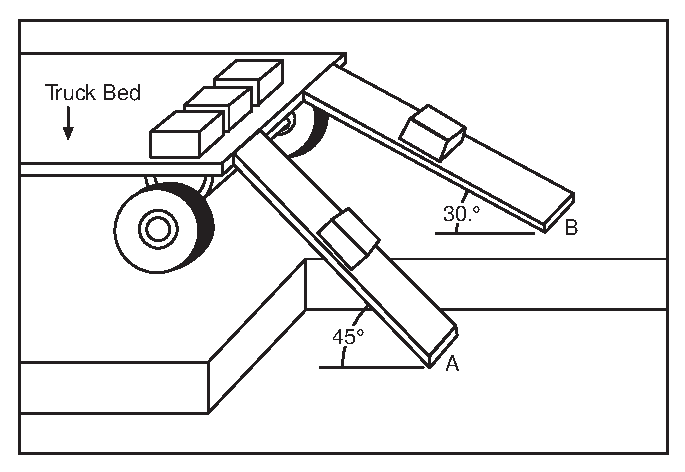
\includegraphics[keepaspectratio,scale=0.66]{Jan2001-Q17}
    \end{center}
    Compared to the amount of work done against friction by a block sliding down plank $A$,
        the work done against friction by a block sliding down plank $B$ is:
    \begin{multicols}{2}
    \begin{choices}
        \wrongchoice{less}
      \correctchoice{more}
        \wrongchoice{the same}
    \end{choices}
    \end{multicols}
\end{question}
}

\element{nysed}{
\begin{question}{Jan2001-Q18}
    Two vacationers walk out on a horizontal pier as shown in the diagram below.
    \begin{center}
        %% NOTE: very complex, keep
        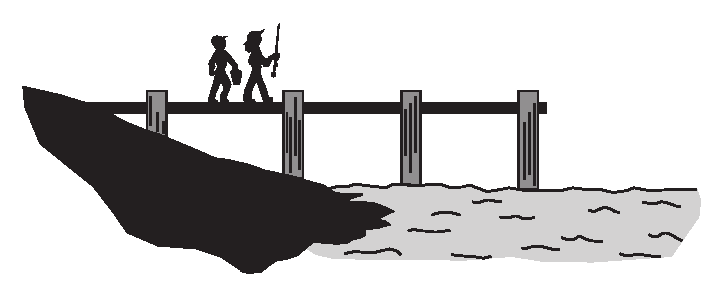
\includegraphics[keepaspectratio,scale=0.66]{Jan2001-Q18}
    \end{center}
    As they approach the end of the pier,
        their gravitational potential energy will
    \begin{multicols}{2}
    \begin{choices}
        \wrongchoice{decrease}
        \wrongchoice{increase}
      \correctchoice{remain the same}
    \end{choices}
    \end{multicols}
\end{question}
}

\element{nysed}{
\begin{question}{Jan2001-Q20}
    The graph below represents the elongation of a spring as a function of the applied force.
    \begin{center}
    \begin{tikzpicture}
        \begin{axis}[
            axis y line=left,
            axis x line=bottom,
            axis line style={->},
            xlabel={elongation},
            xtick={0,0.1,0.2,0.3,0.4},
            x unit=\si{\meter},
            ylabel={force},
            y unit=\si{\newton},
            ytick={0,6,12,18,24},
            xmin=0,xmax=0.45,
            ymin=0,ymax=27,
            grid=major,
            width=0.8\columnwidth,
            height=0.5\columnwidth,
            very thin,
        ]
        \addplot[line width=1pt,domain=0:0.41]{60*x};
        \end{axis}
    \end{tikzpicture}
    \end{center}
    How much work must be done to stretch the spring \SI{0.40}{\meter}?
    \begin{multicols}{2}
    \begin{choices}
      \correctchoice{\SI{4.8}{\joule}}
        \wrongchoice{\SI{6.0}{\joule}}
        \wrongchoice{\SI{9.8}{\joule}}
        \wrongchoice{\SI{24}{\joule}}
    \end{choices}
    \end{multicols}
\end{question}
}


%% Section June2000
%%--------------------
\element{nysed}{
\begin{question}{June2000-Q18}
    A student applies a \SI{20}{\newton} force to move a crate at a constant speed of \SI{4.0}{\meter\per\second} across a rough floor.
    How much work is done by the student on the crate in \SI{6.0}{\second}?
    \begin{multicols}{2}
    \begin{choices}
        \wrongchoice{\SI{80}{\joule}}
        \wrongchoice{\SI{120}{\joule}}
        \wrongchoice{\SI{240}{\joule}}
      \correctchoice{\SI{480}{\joule}}
    \end{choices}
    \end{multicols}
\end{question}
}

\element{nysed}{
\begin{question}{June2000-Q21}
    The kinetic energy of a \SI{980}{\kilo\gram} race car traveling at \SI{90}{\meter\per\second} is approximately:
    \begin{multicols}{2}
    \begin{choices}
        \wrongchoice{\SI{4.4e4}{\joule}}
        \wrongchoice{\SI{8.8e4}{\joule}}
      \correctchoice{\SI{4.0e6}{\joule}}
        \wrongchoice{\SI{7.9e6}{\joule}}
    \end{choices}
    \end{multicols}
\end{question}
}

\element{nysed}{
\begin{question}{June2000-Q29}
    In the diagram below, a student compressed the spring in a pop-up toy \SI{0.020}{\meter}.
    %% I changed the graph as the original did not make sense
    \begin{center}
    \begin{tikzpicture}
        \begin{axis}[
            axis y line=left,
            axis x line=bottom,
            axis line style={->},
            xlabel={compression},
            xtick=\empty,
            ylabel={force},
            ytick=\empty,
            xmin=0,xmax=10,
            ymin=0,ymax=10,
            grid=major,
            width=0.90\columnwidth,
            height=0.40\columnwidth,
            very thin,
        ]
        \addplot[line width=1pt,domain=0:10]{x};
        \end{axis}
    \end{tikzpicture}
    \end{center}
    If the spring has a spring constant of \SI{340}{\newton\per\meter},
        how much energy is being stored in the spring?
    \begin{multicols}{2}
    \begin{choices}
      \correctchoice{\SI{0.068}{\joule}}
        \wrongchoice{\SI{0.14}{\joule}}
        \wrongchoice{\SI{3.4}{\joule}}
        \wrongchoice{\SI{6.8}{\joule}}
    \end{choices}
    \end{multicols}
\end{question}
}


%% Section June1999
%%--------------------
\element{nysed}{
\begin{question}{June1999-Q19}
    A girl rides an escalator that moves her upward at constant speed.
    As the girl rises,
        how does her gravitational potential energy and kinetic energy change?
    \begin{choices}
        \wrongchoice{Gravitational potential energy decreases and kinetic energy decreases.}
        \wrongchoice{Gravitational potential energy decreases and kinetic energy remains the same.}
        \wrongchoice{Gravitational potential energy increases and kinetic energy decreases.}
      \correctchoice{Gravitational potential energy increases and kinetic energy remains the same.}
    \end{choices}
\end{question}
}

\element{nysed}{
\begin{question}{June1999-Q20}
    A student does \SI{300}{\joule} of work pushing a cart \SI{3.0}{\meter} due east and then does \SI{400}{\joule} of work pushing the cart \SI{4.0}{\meter} due north.
    The total amount of work done by the student is:
    \begin{multicols}{2}
    \begin{choices}
        \wrongchoice{\SI{100}{\joule}}
        \wrongchoice{\SI{500}{\joule}}
      \correctchoice{\SI{700}{\joule}}
        \wrongchoice{\SI{2500}{\joule}}
    \end{choices}
    \end{multicols}
\end{question}
}

\element{nysed}{
\begin{question}{June1999-Q21}
    The unstretched spring in the diagram below has a length of \SI{0.40}{\meter} and spring constant $k$.
    A weight is hung from the spring, causing it to stretch to a length of \SI{0.60}{\meter}.
    \begin{center}
    \begin{tikzpicture}
        \begin{scope}[xshift=-2cm]
            %% Title
            \node[anchor=south,text centered] at (0.5,0.2cm) {Unstretched};
            %% Celiing
            \draw (-1,0) --  (2,0);
            \node[anchor=south,fill,pattern=north east lines,minimum width=3cm, minimum height=0.05cm] at (0.5,0) {};
            %% Spring
            \draw[thick,decoration={aspect=0.2,segment length=2mm,amplitude=4mm,coil},decorate] (0,0) -- (0,-2);
            \draw[dashed]  (0,-2) -- ++(0:1cm);
            %% Ruler
            \draw[<->] (1.5,0) -- (1.5,-2) node[pos=0.5,anchor=center,fill=white] {\SI{0.40}{\meter}};
        \end{scope}
        \begin{scope}[xshift=+2cm]
            %% Title
            \node[anchor=south,text centered] at (0.5,0.2cm) {Stretched};
            %% Celiing
            \draw (-1,0) --  (2,0);
            \node[anchor=south,fill,pattern=north east lines,minimum width=3cm, minimum height=0.05cm] at (0.5,0) {};
            %% Weight
            \node[anchor=north,draw,minimum size=1cm] (M) at (0,-3) {Weight};
            %% Spring
            \draw[thick,decoration={aspect=0.2,segment length=3mm,amplitude=4mm,coil},decorate] (0,0) -- (0,-3);
            \draw[dashed]  (0,-3) -- ++(0:1cm);
            %% Ruler
            \draw[<->] (1.5,0) -- (1.5,-3) node[pos=0.5,anchor=center,fill=white] {\SI{0.60}{\meter}};
        \end{scope}
    \end{tikzpicture}
    \end{center}
    How many joules of elastic potential energy are stored in this stretched spring?
    \begin{multicols}{2}
    \begin{choices}
      \correctchoice{$0.020\times k$}
        \wrongchoice{$0.080\times k$}
        \wrongchoice{$0.18\times k$}
        \wrongchoice{$2.0\times k$}
        %% NOTE: 0.2 would be better distrator
    \end{choices}
    \end{multicols}
\end{question}
}

\element{nysed}{
\begin{question}{June1999-Q22}
    A spring has a spring constant of \SI{25}{\newton\per\meter}.
    The minimum force required to stretch the spring \SI{0.25}{\meter} from its equilibrium position is approximately:
    \begin{multicols}{2}
    \begin{choices}
        \wrongchoice{\SI{1.0e-4}{\newton}}
        \wrongchoice{\SI{0.78}{\newton}}
      \correctchoice{\SI{6.3}{\newton}}
        \wrongchoice{\SI{1.0e2}{\newton}}
    \end{choices}
    \end{multicols}
\end{question}
}

%% NOTE: June1999-Q24 requires graphics
%% NOTE: cannot extract vector graphic
%\element{nysed}{
%\begin{question}{June1999-Q24}
%    In the diagram below, an average force of \SI{20}{\newton}
%        is used to pull back the string of a bow \SI{0.60}{\meter}.
%    \begin{center}
%        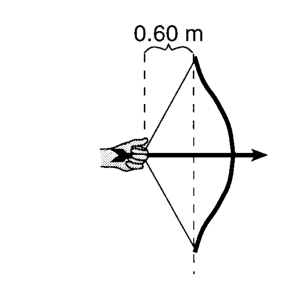
\includegraphics[keepaspectratio,scale=0.75]{June1999-Q24}
%    \end{center}
%    The arrow leaves the bow, its kinetic energy is:
%    \begin{multicols}{2}
%    \begin{choices}
%        \wrongchoice{\SI{3.4}{\joule}}
%        \wrongchoice{\SI{6.0}{\joule}}
%        \wrongchoice{\SI{12}{\joule}}
%        \wrongchoice{\SI{33}{\joule}}
%    \end{choices}
%    \end{multicols}
%\end{question}
%}


%% Section June1998
%%--------------------
\element{nysed}{
\begin{question}{June1998-Q14}
    If the speed of a moving object is doubled,
        which quantity associated with the object must also double?
    \begin{choices}
      \correctchoice{its momentum}
        \wrongchoice{its kinetic energy}
        \wrongchoice{its acceleration}
        \wrongchoice{its gravitational potential energy}
    \end{choices}
\end{question}
}

\element{nysed}{
\begin{question}{June1998-Q18}
    Which action would require no work to be done on an object?
    \begin{choices}
        \wrongchoice{lifting the object from the floor to the ceiling}
        \wrongchoice{pushing the object along a horizontal floor against a frictional force}
        \wrongchoice{decreasing the speed of the object until it comes to rest}
      \correctchoice{holding the object stationary above the ground}
    \end{choices}
\end{question}
}

\element{nysed}{
\begin{question}{June1998-Q20}
    A \SI{60}{\kilo\gram} student running at \SI{3.0}{\meter\per\second} has a kinetic energy of:
    \begin{multicols}{2}
    \begin{choices}
        \wrongchoice{\SI{180}{\joule}}
      \correctchoice{\SI{270}{\joule}}
        \wrongchoice{\SI{540}{\joule}}
        \wrongchoice{\SI{8100}{\joule}}
    \end{choices}
    \end{multicols}
\end{question}
}

\element{nysed}{
\begin{question}{June1998-Q21}
    A student pulls a box across a horizontal floor at a constant speed of \SI{4.0}{\meter\per\second} by exerting a constant horizontal force of \SI{45}{\newton}.
    Approximately how much work does the student do against friction in moving the box \SI{5.5}{\meter} across the floor?
    \begin{multicols}{2}
    \begin{choices}
        \wrongchoice{\SI{45}{\joule}}
        \wrongchoice{\SI{180}{\joule}}
      \correctchoice{\SI{250}{\joule}}
        \wrongchoice{\SI{740}{\joule}}
    \end{choices}
    \end{multicols}
\end{question}
}


%% Section June1997
%%--------------------
\element{nysed}{
\begin{question}{June1997-Q16}
    How much work is done on a downhill skier by an average braking force of \SI{9.8e2}{\newton} to stop her in a distance of \SI{10}{\meter}?
    \begin{multicols}{2}
    \begin{choices}
        \wrongchoice{\SI{1.0e1}{\joule}}
        \wrongchoice{\SI{9.8e1}{\joule}}
        \wrongchoice{\SI{1.0e3}{\joule}}
      \correctchoice{\SI{9.8e3}{\joule}}
    \end{choices}
    \end{multicols}
\end{question}
}

\element{nysed}{
\begin{question}{June1997-Q18}
    A spring has a spring constant of \SI{120}{\newton\per\meter}.
    How much potential energy is stored in the spring as it is stretched \SI{0.20}{\meter}?
    \begin{multicols}{2}
    \begin{choices}
      \correctchoice{\SI{2.4}{\joule}}
        \wrongchoice{\SI{4.8}{\joule}}
        \wrongchoice{\SI{12}{\joule}}
        \wrongchoice{\SI{24}{\joule}}
    \end{choices}
    \end{multicols}
\end{question}
}

\element{nysed}{
\begin{question}{June1997-Q21}
    A cart of mass $M$ on a frictionless track starts from rest at the top of the hill having height $h_1$,
        as shown in the diagram below.
    \begin{center}
    \begin{tikzpicture}[font=\small]
        %% Ground
        \draw[dashed] (-1,0) -- (7,0);
        %% Path
        \draw[thick] (-1,3) -- (0,3) to[out=0,in=180] (2,0) to[out=0,in=180] (4,2) to [out=0,in=180] (5.5,0.75) -- (7,0.75);
        %% Mass
        \node[draw,fill=white!90!black,minimum size=0.5cm,anchor=south] (M) at (0,3.1) {$M$};
        \draw (M.south west) ++(0:0.1) arc (90:-270:0.05);
        \draw (M.south east) ++(180:0.1) arc (90:-270:0.05);
        %% Labels
        \draw[<->] (0,0) -- (0,3) node[pos=0.5,fill=white,anchor=center] {$h_1$};
        \draw[<->] (4,0) -- (4,2) node[pos=0.5,fill=white,anchor=center] {$h_2$};
        \draw[<->] (6,0) -- (6,0.75) node[pos=0.5,anchor=west] {$h_3$};
    \end{tikzpicture}
    \end{center}
    What is the kinetic energy of the cart when it reaches the top of the next hill,
        having height $h_2$?
    \begin{multicols}{2}
    \begin{choices}
        \wrongchoice{$Mgh_1$}
      \correctchoice{$Mg\left(h_1-h_2\right)$}
        \wrongchoice{$Mg\left(h_2-h_3\right)$}
        \wrongchoice{zero}
    \end{choices}
    \end{multicols}
\end{question}
}


%% Section June1996
%%--------------------
\element{nysed}{
\begin{question}{June1996-Q18}
    A box weighing \SI{1.0e2}{\newton} is dragged to the top of an incline,
        as shown in the diagram below.
    \begin{center}
    \begin{tikzpicture}[scale=0.66,font=\small]
        %% Triangle
        \draw[thick] (0,0) -- (8,0) -- (8,6) -- cycle;
        %% Labels
        \draw[<->,thick] (0,-2em) -- (8,-2em) node[pos=0.5,anchor=center,fill=white] {\SI{8}{\meter}};
        \draw[<->,thick] (8cm+3em,0) -- (8cm+3em,6) node[pos=0.5,anchor=center,fill=white] {\SI{6}{\meter}};
        \draw[<->,thick] (126.87:2.5) -- ++(36.87:10) node[pos=0.5,anchor=center,rotate=36.87,fill=white] {\SI{10}{\meter}};
        %% block
        \node[draw,thick,minimum size=1cm,fill=white!90!black,rounded corners=0.5ex,rotate=36.87,anchor=south west] (A) at (36.87:0.01cm) {\SI{e2}{\newton}};
        \draw[thick,->] (A.east) -- ++(36.87:2);
    \end{tikzpicture}
    \end{center}
    The gravitational potential energy of the box at the top of the incline is approximately:
    \begin{multicols}{2}
    \begin{choices}
        \wrongchoice{\SI{1.0e2}{\joule}}
      \correctchoice{\SI{6.0e2}{\joule}}
        \wrongchoice{\SI{8.0e2}{\joule}}
        \wrongchoice{\SI{1.0e3}{\joule}}
    \end{choices}
    \end{multicols}
\end{question}
}

\element{nysed}{
\begin{question}{June1996-Q21}
    Spring $A$ has a spring constant of \SI{140}{\newton\per\meter},
        and spring $B$ has spring constant of \SI{280}{\newton\per\meter}.
    Both springs are stretched at the same distance.
    Compared to the potential energy stored in spring $A$,
        the potential energy stored in spring $B$ is:
    \begin{choices}
        \wrongchoice{the same}
      \correctchoice{twice as great}
        \wrongchoice{half as great}
        \wrongchoice{four times as great}
    \end{choices}
\end{question}
}

\element{nysed}{
\begin{question}{June1996-Q22}
    A cart of mass $m$ traveling at speed $v$ has kinetic energy $KE$.
    If the mass of the cart is doubled and its speed is halved,
        the kinetic energy of the cart will be:
    \begin{choices}
      \correctchoice{half as great}
        \wrongchoice{twice as great}
        \wrongchoice{one-fourth as great}
        \wrongchoice{four times as great}
    \end{choices}
\end{question}
}


%% Section June1996
%%--------------------
\element{nysed}{
\begin{question}{June1995-Q15}
    A constant force of \SI{2.0}{\newton} is used to push a \SI{3.0}{\kilo\gram} mass \SI{4.0}{\meter} across the floor.
    How much work is done on the mass?
    \begin{multicols}{2}
    \begin{choices}
        \wrongchoice{\SI{6.0}{\joule}}
      \correctchoice{\SI{8.0}{\joule}}
        \wrongchoice{\SI{12}{\joule}}
        \wrongchoice{\SI{24}{\joule}}
    \end{choices}
    \end{multicols}
\end{question}
}

\element{nysed}{
\begin{question}{June1995-Q17}
    When a spring is stretched \SI{0.200}{\meter} from its equilibrium position,
        it possesses a potential energy of \SI{10.0}{\joule}.
    What is the spring constant for this spring?
    \begin{multicols}{2}
    \begin{choices}
        \wrongchoice{\SI{100}{\newton\per\meter}}
        \wrongchoice{\SI{125}{\newton\per\meter}}
        \wrongchoice{\SI{250}{\newton\per\meter}}
      \correctchoice{\SI{500}{\newton\per\meter}}
    \end{choices}
    \end{multicols}
\end{question}
}

\element{nysed}{
\begin{question}{June1995-Q18}
    A \SI{1.0e3}{\kilo\gram} car is moving at a constant speed of \SI{4.0}{\meter\per\second}.
    What is the kinetic energy of the car?
    \begin{multicols}{2}
    \begin{choices}
        \wrongchoice{\SI{1.6e3}{\joule}}
        \wrongchoice{\SI{2.0e4}{\joule}}
      \correctchoice{\SI{8.0e3}{\joule}}
        \wrongchoice{\SI{4.0e3}{\joule}}
    \end{choices}
    \end{multicols}
\end{question}
}

\element{nysed}{
\begin{question}{June1995-Q19}
    A force is applied to a block, causing it to accelerate along a horizontal, frictionless surface.
    The energy gained by the block is equal to the:
    \begin{choices}
      \correctchoice{work done on the block}
        \wrongchoice{power applied to the block}
        \wrongchoice{impulse applied to the block}
        \wrongchoice{momentum given to the block}
    \end{choices}
\end{question}
}

\element{nysed}{
\begin{question}{June1995-Q20}
    A \SI{1.0}{\kilo\gram} mass gains kinetic energy as it falls freely from rest a vertical distance, $d$.
    How far would a \SI{2.0}{\kilo\gram} mass have to fall freely from rest to gain the same amount of kinetic energy?
    \begin{multicols}{4}
    \begin{choices}
        \wrongchoice{$d$}
        \wrongchoice{$2d$}
      \correctchoice{$\dfrac{d}{2}$}
        \wrongchoice{$\dfrac{d}{4}$}
    \end{choices}
    \end{multicols}
\end{question}
}


%% Section June1994
%%--------------------
\element{nysed}{
\begin{question}{June1994-Q19}
    Graphs $A$ and $B$ below represent the result of applying an increasing force to stretch a spring which did not exceed its elastic limit.
    \begin{center}
    \begin{tikzpicture}
        \begin{groupplot}[
                axis y line=left,
                axis x line=bottom,
                axis line style={->},
                group style={group size=2 by 1},
                xtick=\empty,
                ytick=\empty,
                xmin=0,xmax=11,
                ymin=0,ymax=11,
                ylabel={Force Applied},
                width=0.5\columnwidth,
            ]
            \nextgroupplot[
                title=$A$,
                xlabel={Spring Displacement},
            ] \addplot[line width=1pt,domain=0:10] {x};
            \nextgroupplot[
                title=$B$,
                xlabel={Work Done on Spring},
            ] \addplot[line width=1pt,domain=0:10] {sqrt(10)*sqrt(x)};
        \end{groupplot}
    \end{tikzpicture}
    \end{center}
    The spring constant can be represented by the:
    \begin{choices}
      \correctchoice{slope of graph $A$}
        \wrongchoice{slope of graph $B$}
        \wrongchoice{reciprocal of the slope of graph $A$}
        \wrongchoice{reciprocal of the slope of graph $B$}
    \end{choices}
\end{question}
}

\element{nysed}{
\begin{question}{June1994-Q20}
    A force of \SI{0.2}{\newton} is needed to compress a spring a distance of \SI{0.02}{\meter}.
    The potential energy stored in this compressed spring is:
    \begin{multicols}{2}
    \begin{choices}
        \wrongchoice{\SI{8e-5}{\joule}}
      \correctchoice{\SI{2e-3}{\joule}}
        \wrongchoice{\SI{2e-5}{\joule}}
        \wrongchoice{\SI{4e-5}{\joule}}
    \end{choices}
    \end{multicols}
\end{question}
}

\element{nysed}{
\begin{question}{June1994-Q21}
    An object with a speed of \SI{20}{\meter\per\second} has a kinetic energy of \SI{400}{\joule}.
    The mass of the object is:
    \begin{multicols}{2}
    \begin{choices}
        \wrongchoice{\SI{1.0}{\kilo\gram}}
      \correctchoice{\SI{2.0}{\kilo\gram}}
        \wrongchoice{\SI{0.50}{\kilo\gram}}
        \wrongchoice{\SI{40}{\kilo\gram}}
    \end{choices}
    \end{multicols}
\end{question}
}



%% Section June1990
%%--------------------
\element{nysed}{
\begin{question}{June1990-Q18}
    The graph below shows the force exerted on a block as a function of the block's displacement in the direction of the force.
    \begin{center}
    \begin{tikzpicture}
        \begin{axis}[
            axis y line=left,
            axis x line=bottom,
            axis line style={->},
            xlabel={displacement},
            x unit=\si{\meter},
            xtick={0,1,2,3,4,5,6,7},
            ylabel={force},
            y unit=\si{\newton},
            ytick={0,2,4,6,8},
            xmin=0,xmax=7.2,
            ymin=0,ymax=8.2,
            width=0.8\columnwidth,
            height=0.5\columnwidth,
            very thin,
        ]
        \addplot[line width=1pt,domain=0:10]{4};
        \end{axis}
    \end{tikzpicture}
    \end{center}
    How much work did the force do in displacing the block \SI{5.0}{\meter}?
    \begin{multicols}{2}
    \begin{choices}
        \wrongchoice{\SI{0}{\joule}}
      \correctchoice{\SI{20}{\joule}}
        \wrongchoice{\SI{0.80}{\joule}}
        \wrongchoice{\SI{4.0}{\joule}}
    \end{choices}
    \end{multicols}
\end{question}
}

\element{nysed}{
\begin{question}{June1990-Q20}
    When a \SI{5}{\kilo\gram} mass is lifted from ground to a height of \SI{10}{\meter},
        the gravitational potential energy of the mass is increased by approximately:
    \begin{multicols}{2}
    \begin{choices}
        \wrongchoice{\SI{0.5}{\joule}}
        \wrongchoice{\SI{2}{\joule}}
        \wrongchoice{\SI{50}{\joule}}
      \correctchoice{\SI{500}{\joule}}
    \end{choices}
    \end{multicols}
\end{question}
}

\element{nysed}{
\begin{question}{June1990-Q21}
    If the speed of an object is doubled,
        its kinetic energy will be:
    \begin{multicols}{2}
    \begin{choices}
        \wrongchoice{halved}
        \wrongchoice{doubled}
        \wrongchoice{quartered}
      \correctchoice{quadrupled}
    \end{choices}
    \end{multicols}
\end{question}
}

\element{nysed}{
\begin{question}{June1990-Q23}
    An object \SI{10}{\meter} above the ground has $Z$ joules of potential energy.
    If the object falls freely,
        how many joules of kinetic energy will it have gained when it is \SI{5}{\meter} above the ground?
    \begin{multicols}{2}
    \begin{choices}
        \wrongchoice{$Z$}
        \wrongchoice{$2Z$}
      \correctchoice{$\dfrac{Z}{2}$}
        \wrongchoice{zero}
    \end{choices}
    \end{multicols}
\end{question}
}


%% Section June1989
%%--------------------
\element{nysed}{
\begin{question}{June1989-Q23}
    An object gains \SI{10}{\joule} of potential energy as it is lifted vertically \SI{2.0}{\meter}.
    If a second object with one-half the mass is lifted vertically \SI{2.0}{\meter},
        the potential energy gained by the second object will be:
    \begin{multicols}{2}
    \begin{choices}
        \wrongchoice{\SI{10}{\joule}}
        \wrongchoice{\SI{20}{\joule}}
      \correctchoice{\SI{5.0}{\joule}}
        \wrongchoice{\SI{2.5}{\joule}}
    \end{choices}
    \end{multicols}
\end{question}
}

\element{nysed}{
\begin{question}{June1989-Q24}
    A spring of negligible mass with a spring constant of \SI{200}{\newton\per\meter} is stretched \SI{0.2}{\meter}.
    How much potential energy is stored in the spring?
    \begin{multicols}{2}
    \begin{choices}
        \wrongchoice{\SI{40}{\joule}}
        \wrongchoice{\SI{20}{\joule}}
        \wrongchoice{\SI{8}{\joule}}
      \correctchoice{\SI{4}{\joule}}
    \end{choices}
    \end{multicols}
\end{question}
}

\element{nysed}{
\begin{question}{June1989-Q25}
    Which graph best represents the relationship between the kinetic energy (KE) of a moving object as a function of its velocity?
    \begin{multicols}{2}
    \begin{choices}
        \AMCboxDimensions{down=-2.5em}
        \wrongchoice{
            \begin{tikzpicture}
                \begin{axis}[
                    axis y line=left,
                    axis x line=bottom,
                    axis line style={->},
                    xlabel={KE},
                    xtick=\empty,
                    ylabel={velocity},
                    ytick=\empty,
                    xmin=0,xmax=11,
                    ymin=0,ymax=11,
                    width=\columnwidth,
                    very thin,
                ]
                \addplot[line width=1pt,domain=0:10]{8};
                \end{axis}
            \end{tikzpicture}
        }
        \wrongchoice{
            \begin{tikzpicture}
                \begin{axis}[
                    axis y line=left,
                    axis x line=bottom,
                    axis line style={->},
                    xlabel={KE},
                    xtick=\empty,
                    ylabel={velocity},
                    ytick=\empty,
                    xmin=0,xmax=11,
                    ymin=0,ymax=11,
                    width=\columnwidth,
                    very thin,
                ]
                \addplot[line width=1pt,domain=0:10]{x};
                \end{axis}
            \end{tikzpicture}
        }
        %% ANS is 3
        \correctchoice{
            \begin{tikzpicture}
                \begin{axis}[
                    axis y line=left,
                    axis x line=bottom,
                    axis line style={->},
                    xlabel={KE},
                    xtick=\empty,
                    ylabel={velocity},
                    ytick=\empty,
                    xmin=0,xmax=11,
                    ymin=0,ymax=11,
                    width=\columnwidth,
                    very thin,
                ]
                \addplot[line width=1pt,domain=0:10]{0.1*x*x};
                \end{axis}
            \end{tikzpicture}
        }
        \wrongchoice{
            \begin{tikzpicture}
                \begin{axis}[
                    axis y line=left,
                    axis x line=bottom,
                    axis line style={->},
                    xlabel={KE},
                    xtick=\empty,
                    ylabel={velocity},
                    ytick=\empty,
                    xmin=0,xmax=11,
                    ymin=0,ymax=11,
                    width=\columnwidth,
                    very thin,
                ]
                \addplot[line width=1pt,domain=0:10]{10/x};
                \end{axis}
            \end{tikzpicture}
        }
    \end{choices}
    \end{multicols}
\end{question}
}

\element{nysed}{
\begin{question}{June1989-Q26}
    A basketball player who weighs \SI{600}{\newton} jumps \SI{0.5}{\meter} vertically off the floor.
    What is her kinetic energy just before hitting the floor?
    \begin{multicols}{2}
    \begin{choices}
        \wrongchoice{\SI{30}{\joule}}
        \wrongchoice{\SI{60}{\joule}}
      \correctchoice{\SI{300}{\joule}}
        \wrongchoice{\SI{600}{\joule}}
    \end{choices}
    \end{multicols}
\end{question}
}


%% Section June1986
%%--------------------
\element{nysed}{
\begin{question}{June1986-Q13}
    A \SI{2.2}{\kilo\gram} mass is pulled by a \SI{30}{\newton} force through a distance of \SI{5.0}{\meter} as shown in the diagram below.
    \begin{center}
    \begin{tikzpicture}
        %% ground
        \draw (-3.5,0) -- (3.5,0);
        \node[anchor=north,minimum width=7cm,pattern=north east lines] at (0,0) {};
        %% box
        \node[anchor=south,draw,minimum size=1cm] (A) at (-1,0) {\SI{2.2}{\kilo\gram}};
        \draw[thick,-latex] (A.east) -- ++(0:2) node[pos=0.5,anchor=south] {\SI{30}{\newton}};
        %% distance
        \draw[dashed] (A.north east) -- ++(90:1);
        \draw[<->] (A.north east) ++(90:0.75) -- ++(0:3) node[pos=0.5,anchor=center,fill=white] {\SI{50}{\meter}};
        \draw[dashed] (A.north east) ++ (90:1) ++ (0:3) -- ++(270:1);
    \end{tikzpicture}
    \end{center}
    What amount of work is done?
    \begin{multicols}{2}
    \begin{choices}
        \wrongchoice{\SI{11}{\joule}}
        \wrongchoice{\SI{66}{\joule}}
      \correctchoice{\SI{150}{\joule}}
        \wrongchoice{\SI{330}{\joule}}
    \end{choices}
    \end{multicols}
\end{question}
}

\element{nysed}{
\begin{question}{June1986-Q14}
    A mass resting on a shelf \SI{10.0}{\meter} above the floor has a gravitational potential energy of \SI{980}{\joule} with respect to the floor.
    The mass is moved to a shelf \SI{8.00}{\meter} above the floor.
    What is the new gravitational potential energy?
    \begin{multicols}{2}
    \begin{choices}
        \wrongchoice{\SI{960}{\joule}}
      \correctchoice{\SI{784}{\joule}}
        \wrongchoice{\SI{490}{\joule}}
        \wrongchoice{\SI{196}{\joule}}
    \end{choices}
    \end{multicols}
\end{question}
}

\element{nysed}{
\begin{question}{June1986-Q16}
    Which cart shown below has the greatest kinetic energy?
    \begin{multicols}{2}
    \begin{choices}
        \AMCboxDimensions{down=-0.4cm}
        %% NOTE: ANS is 2
        \wrongchoice{
            \begin{tikzpicture}
                \draw[dashed,white!60!black] (-1.5,-0.5) rectangle (1.5,2.5);
                %% ground
                \draw (-1.5,0) -- (1.5,0);
                \node[anchor=north,minimum width=3cm,pattern=north east lines] at (0,0) {};
                %% Cart
                \node[draw,minimum height=1.0cm,minimum width=2.0cm,anchor=south] (L) at (0,0.2) {\SI{1}{\kilo\gram}};
                \draw[fill=white] (L.south west) ++(0:0.3) circle (0.2);
                \draw[fill=black] (L.south west) ++(0:0.3) circle (1pt);
                \draw[fill=white] (L.south east) ++(180:0.3) circle (0.2);
                \draw[fill=black] (L.south east) ++(180:0.3) circle (1pt);
                \draw[thick,->] (L.north west) ++(90:1em) -- ++(0:2cm) node[pos=0.5,anchor=south] {\SI{4}{\meter\per\second}};
            \end{tikzpicture}
        }
        \wrongchoice{
            \begin{tikzpicture}
                \draw[dashed,white!60!black] (-1.5,-0.5) rectangle (1.5,2.5);
                %% ground
                \draw (-1.5,0) -- (1.5,0);
                \node[anchor=north,minimum width=3cm,pattern=north east lines] at (0,0) {};
                %% Cart
                \node[draw,minimum height=1.0cm,minimum width=2.0cm,anchor=south] (L) at (0,0.2) {\SI{2}{\kilo\gram}};
                \draw[fill=white] (L.south west) ++(0:0.3) circle (0.2);
                \draw[fill=black] (L.south west) ++(0:0.3) circle (1pt);
                \draw[fill=white] (L.south east) ++(180:0.3) circle (0.2);
                \draw[fill=black] (L.south east) ++(180:0.3) circle (1pt);
                \draw[thick,->] (L.north west) ++(90:1em) -- ++(0:2cm) node[pos=0.5,anchor=south] {\SI{3}{\meter\per\second}};
            \end{tikzpicture}
        }
        \wrongchoice{
            \begin{tikzpicture}
                \draw[dashed,white!60!black] (-1.5,-0.5) rectangle (1.5,2.5);
                %% ground
                \draw (-1.5,0) -- (1.5,0);
                \node[anchor=north,minimum width=3cm,pattern=north east lines] at (0,0) {};
                %% Cart
                \node[draw,minimum height=1.0cm,minimum width=2.0cm,anchor=south] (L) at (0,0.2) {\SI{3}{\kilo\gram}};
                \draw[fill=white] (L.south west) ++(0:0.3) circle (0.2);
                \draw[fill=black] (L.south west) ++(0:0.3) circle (1pt);
                \draw[fill=white] (L.south east) ++(180:0.3) circle (0.2);
                \draw[fill=black] (L.south east) ++(180:0.3) circle (1pt);
                \draw[thick,->] (L.north east) ++(90:1em) -- ++(180:2cm) node[pos=0.5,anchor=south] {\SI{2}{\meter\per\second}};
            \end{tikzpicture}
        }
        \wrongchoice{
            \begin{tikzpicture}
                \draw[dashed,white!60!black] (-1.5,-0.5) rectangle (1.5,2.5);
                %% ground
                \draw (-1.5,0) -- (1.5,0);
                \node[anchor=north,minimum width=3cm,pattern=north east lines] at (0,0) {};
                %% Cart
                \node[draw,minimum height=1.0cm,minimum width=2.0cm,anchor=south] (L) at (0,0.2) {\SI{4}{\kilo\gram}};
                \draw[fill=white] (L.south west) ++(0:0.3) circle (0.2);
                \draw[fill=black] (L.south west) ++(0:0.3) circle (1pt);
                \draw[fill=white] (L.south east) ++(180:0.3) circle (0.2);
                \draw[fill=black] (L.south east) ++(180:0.3) circle (1pt);
                \draw[thick,->] (L.north east) ++(90:1em) -- ++(180:2cm) node[pos=0.5,anchor=south] {\SI{1}{\meter\per\second}};
            \end{tikzpicture}
        }
    \end{choices}
    \end{multicols}
\end{question}
}


%% Section June1985
%%--------------------
\element{nysed}{
\begin{question}{June1985-Q11}
    A \SI{1.0}{\kilo\gram} mass falls a distance of \SI{0.50}{\meter},
        causing a \SI{2.0}{\kilo\gram} mass to slide the same distance along a table top,
        as represented in the diagram below.
    \begin{center}
    \begin{tikzpicture}
        %% Floor
        \draw[thick] (-4,0) -- (0,0) -- (0,-2);
        \node[anchor=north,minimum width=4cm,pattern=north east lines] at (-2,0) {};
        %% Mass
        \node[draw,fill=white!90!black,rectangle,rounded corners=1ex,minimum size=1.22cm,anchor=south] (A) at (-3,0) {\SI{2.0}{\kilo\gram}};
        \node[draw,fill=white!90!black,rectangle,rounded corners=1ex,minimum size=1.00cm,anchor=north] (B) at (1,-0.5) {\SI{1.0}{\kilo\gram}};
        %% Rope and Pulley
        \draw[thick] (A.south east) ++(90:0.5) -- (0.75,0.5) arc(90:0:0.25) -- (B.north);
        \draw[thick,fill=white!90!black] (0.75,0.25) circle (0.25);
        \draw[thick,fill=white] (0,0) -- (0.75,0.35) arc (90:-60:0.1) -- (0,-0.5) -- cycle;
        \draw[fill] (0.75,0.25) circle (1pt);
        %% distance
        \draw[<->] (B.south) -- ++(270:2) node[pos=0.5,anchor=center,fill=white] {\SI{0.50}{\meter}};
        \draw (B.south) ++ (270:2) -- ++(0:1) -- ++(180:2);
        \path (B.south) ++ (270:2) node[anchor=north,minimum width=2cm,pattern=north east lines] {};
    \end{tikzpicture}
    \end{center}
    How much work is done by the falling mass?
    \begin{multicols}{2}
    \begin{choices}
        \wrongchoice{\SI{1.5}{\joule}}
      \correctchoice{\SI{4.9}{\joule}}
        \wrongchoice{\SI{9.8}{\joule}}
        \wrongchoice{\SI{14.7}{\joule}}
    \end{choices}
    \end{multicols}
\end{question}
}

\element{nysed}{
\begin{question}{June1985-Q12}
    Which quantities are measured in the same units?
    \begin{multicols}{2}
    \begin{choices}
        \wrongchoice{mass and weight}
        \wrongchoice{heat and temperature}
        \wrongchoice{power and work}
      \correctchoice{work and energy}
    \end{choices}
    \end{multicols}
\end{question}
}

\element{nysed}{
\begin{question}{June1985-Q13}
    The diagram below represents a cart traveling from left to right along a frictionless surface with an initial speed of $v$.
    \begin{center}
    \begin{tikzpicture}[font=\small]
        %% Path
        \draw[very thick] (-4,3) -- (-2,3) to[out=0,in=180] (0,1) to[out=0,in=180] (2,2) -- (4,2);
        \node[anchor=south east] at (4,2) {Earth's Surface};
        %% Cart
        \node[draw,fill=white!90!black,minimum width=1.25cm,minimum height=0.75cm,anchor=south] (M) at (-3,3.2) {};
        \draw[fill=white] (M.south west) ++(+0.3,0) circle (0.2);
        \draw[fill=black] (M.south west) ++(+0.3,0) circle (1pt);
        \draw[fill=white] (M.south east) ++(-0.3,0) circle (0.2);
        \draw[fill=black] (M.south east) ++(-0.3,0) circle (1pt);
        \draw[thick,-latex] (M.north west) ++(90:2ex) -- ++(0:1.25cm) node[pos=0.5,anchor=south] {$v$};
        %% Labels
        \fill (-2,3) circle (2pt) node[anchor=north] {$A$};
        \fill (0,1) circle (2pt) node[anchor=north] {$B$};
        \fill (1,1.5) circle (2pt) node[anchor=north west] {$C$};
        \fill (2,2) circle (2pt) node[anchor=north] {$D$};
    \end{tikzpicture}
    \end{center}
    At which point is the gravitational potential energy of the car \emph{least}?
    \begin{multicols}{4}
    \begin{choices}[o]
        \wrongchoice{$A$}
      \correctchoice{$B$}
        \wrongchoice{$C$}
        \wrongchoice{$D$}
    \end{choices}
    \end{multicols}
\end{question}
}

\element{nysed}{
\begin{question}{June1985-Q14}
    If the velocity of an automobile is doubled,
        its kinetic energy:
    \begin{choices}
        \wrongchoice{decrease to one-half}
        \wrongchoice{doubles}
        \wrongchoice{decrease to one-fourth}
      \correctchoice{quadruples}
    \end{choices}
\end{question}
}

\element{nysed}{
\begin{question}{June1985-Q57}
    As an object falls freely in a vacuum,
        its total energy:
    \begin{choices}
        \wrongchoice{decreases}
        \wrongchoice{increases}
      \correctchoice{remains the same}
    \end{choices}
\end{question}
}


\endinput


